%%
%% This is file `sample-authordraft.tex',
%% generated with the docstrip utility.
%%
%% The original source files were:
%%
%% samples.dtx  (with options: `authordraft')
%% 
%% IMPORTANT NOTICE:
%% 
%% For the copyright see the source file.
%% 
%% Any modified versions of this file must be renamed
%% with new filenames distinct from sample-authordraft.tex.
%% 
%% For distribution of the original source see the terms
%% for copying and modification in the file samples.dtx.
%% 
%% This generated file may be distributed as long as the
%% original source files, as listed above, are part of the
%% same distribution. (The sources need not necessarily be
%% in the same archive or directory.)
%%
%% The first command in your LaTeX source must be the \documentclass command.
% \documentclass[sigconf,authordraft]{acmart}


%%%% As of March 2017, [siggraph] is no longer used. Please use sigconf (above) for SIGGRAPH conferences.

%%%% As of May 2020, [sigchi] and [sigchi-a] are no longer used. Please use sigconf (above) for SIGCHI conferences.

%%%% Proceedings format for SIGPLAN conferences 
% \documentclass[sigplan, anonymous, authordraft]{acmart}

%%%% Proceedings format for conferences using one-column small layout
\documentclass[acmsmall,authordraft]{acmart}

% NOTE that a single column version is required for submission and peer review. This can be done by changing the \doucmentclass[...]{acmart} in this template to 
% \documentclass[manuscript,screen]{acmart}

%%
%% \BibTeX command to typeset BibTeX logo in the docs
\AtBeginDocument{%
  \providecommand\BibTeX{{%
    \normalfont B\kern-0.5em{\scshape i\kern-0.25em b}\kern-0.8em\TeX}}}

%% Rights management information.  This information is sent to you
%% when you complete the rights form.  These commands have SAMPLE
%% values in them; it is your responsibility as an author to replace
%% the commands and values with those provided to you when you
%% complete the rights form.
\setcopyright{acmcopyright}
\copyrightyear{2018}
\acmYear{2018}
\acmDOI{10.1145/1122445.1122456}

%% These commands are for a PROCEEDINGS abstract or paper.
\acmConference[Woodstock '18]{Woodstock '18: ACM Symposium on Neural
  Gaze Detection}{June 03--05, 2018}{Woodstock, NY}
\acmBooktitle{Woodstock '18: ACM Symposium on Neural Gaze Detection,
  June 03--05, 2018, Woodstock, NY}
\acmPrice{15.00}
\acmISBN{978-1-4503-XXXX-X/18/06}


%%
%% Submission ID.
%% Use this when submitting an article to a sponsored event. You'll
%% receive a unique submission ID from the organizers
%% of the event, and this ID should be used as the parameter to this command.
%%\acmSubmissionID{123-A56-BU3}

%%
%% The majority of ACM publications use numbered citations and
%% references.  The command \citestyle{authoryear} switches to the
%% "author year" style.
%%
%% If you are preparing content for an event
%% sponsored by ACM SIGGRAPH, you must use the "author year" style of
%% citations and references.
%% Uncommenting
%% the next command will enable that style.
%%\citestyle{acmauthoryear}

%%
%% end of the preamble, start of the body of the document source.
\begin{document}

%%
%% The "title" command has an optional parameter,
%% allowing the author to define a "short title" to be used in page headers.
\title[Scientific Knowledge Sharing at Scale During Pandemic]{Testing: Challenges to Large-scale Scientific Knowledge Sharing During the COVID-19 Pandemic}

%%
%% The "author" command and its associated commands are used to define
%% the authors and their affiliations.
%% Of note is the shared affiliation of the first two authors, and the
%% "authornote" and "authornotemark" commands
%% used to denote shared contribution to the research.
\author{Author 1}
\authornote{Note 1}
\email{email@mail.com}
\orcid{1234-5678-9012}
\affiliation{%
  \institution{Institution}
  \streetaddress{P.O. Box 1234}
  \city{City}
  \state{State}
  \postcode{12345-6789}
}

\author{Author 2}
\affiliation{%
  \institution{Institution}
  \streetaddress{P.O. Box 1234}
  \city{City}
  \country{State}}
\email{email@mail.com}


%%
%% By default, the full list of authors will be used in the page
%% headers. Often, this list is too long, and will overlap
%% other information printed in the page headers. This command allows
%% the author to define a more concise list
%% of authors' names for this purpose.
\renewcommand{\shortauthors}{Author 1, et al.}

%%
%% The abstract is a short summary of the work to be presented in the
%% article.
\begin{abstract}
The COVID-19 pandemic poses major challenges to researchers using existing cyberinfrastructures to collaborate and share COVID-19 scientific knowledge. This paper enriches the existing literature by investigating the following challenges: (1) the mass influx of publications imposes a cognitive overload on COVID-19 researchers, (2) increasing speed of publications requires additional efforts to preserve peer-evaluation quality, (3) decentralization of research communities imposes impediments to informing the larger community about inappropriate results/interpretations in papers, (4) rigidity of papers imposes barriers to updating prior findings, and (5) difficulties with establishing common ground make interdisciplinary research more challenging. We manually reviewed approximately $1,300$ tweets about large-scale collaborative research problems. We conducted a thematic analysis of about $10\%$ of these tweets through a grounded theory approach and affinity mapping. We call on the CHI community to design scalable solutions for rapid knowledge sharing that help researchers collaboratively summarize, organize, share, and peer-review/improve their knowledge.
\end{abstract}

%%
%% The code below is generated by the tool at http://dl.acm.org/ccs.cfm.
%% Please copy and paste the code instead of the example below.
%%
\begin{CCSXML}
<ccs2012>
   <concept>
       <concept_id>10003120.10003130.10003131.10003234</concept_id>
       <concept_desc>Human-centered computing~Social content sharing</concept_desc>
       <concept_significance>500</concept_significance>
       </concept>
   <concept>
       <concept_id>10003120.10003130.10003131.10003235</concept_id>
       <concept_desc>Human-centered computing~Collaborative content creation</concept_desc>
       <concept_significance>300</concept_significance>
       </concept>
   <concept>
       <concept_id>10003120.10003130.10003131.10003292</concept_id>
       <concept_desc>Human-centered computing~Social networks</concept_desc>
       <concept_significance>300</concept_significance>
       </concept>
   <concept>
       <concept_id>10003120.10003130.10003131.10003570</concept_id>
       <concept_desc>Human-centered computing~Computer supported cooperative work</concept_desc>
       <concept_significance>500</concept_significance>
       </concept>
   <concept>
       <concept_id>10003120.10003130.10003131.10011761</concept_id>
       <concept_desc>Human-centered computing~Social media</concept_desc>
       <concept_significance>300</concept_significance>
       </concept>
 </ccs2012>
\end{CCSXML}

\ccsdesc[500]{Human-centered computing~Social content sharing}
\ccsdesc[300]{Human-centered computing~Collaborative content creation}
\ccsdesc[300]{Human-centered computing~Social networks}
\ccsdesc[500]{Human-centered computing~Computer supported cooperative work}
\ccsdesc[300]{Human-centered computing~Social media}

%%
%% Keywords. The author(s) should pick words that accurately describe
%% the work being presented. Separate the keywords with commas.
\keywords{E-science, E-research, CSCW, Collaborative Research, COVID-19, Knowledge Graph, Knowledge Sharing}

%% A "teaser" image appears between the author and affiliation
%% information and the body of the document, and typically spans the
%% page.

%%
%% This command processes the author and affiliation and title
%% information and builds the first part of the formatted document.
\maketitle

\section{Introduction}
\label{Introduction}

%motivation for the paper
%why to read

%start with: researchers are working hard to generate knowledge but they are drowining in it and having trouble keeping up

%Needs to be moved: 
There have been numerous studies on scientific data collection, sharing, filtering, analysis, and maintenance in the domains of E-science and CSCW. However, the design community has paid less attention to the dissemination, distillation, organization, and improvement of the result of analyzing, interpreting, and learning through the data, i.e., scientific knowledge. While traditional methods, such as knowledge sharing through journal publications, and classification of publications in knowledge repositories have been relatively efficient in past years, in the wake of the pandemic, new issues have arisen. In this study, we review the recent literature and analyze tweets by COVID-19 researchers explaining the difficulties they experience in scientific knowledge sharing, evaluating, and improving due to the nature of expedited research during the pandemic.

Within the pandemic, there is also an infodemic \citep{WHO2020Munich}. Misinformation about COVID-19 has spread across media platforms \citep{cuan2020misinformation, pennycook2020fighting}, incorporated numerous topics \citep{brennen2020types} and exacerbated public panic \citep{depoux2020pandemic}. While all of this is bad, there exists another underlying cause of the infodemic, taking root in the place where the pursuit of novelty and rigorous evaluation is supposed to prevent misinformation, the inability to effectively share scientific knowledge during the pandemic. 

Due to the massive influx of COVID-19 related knowledge, researchers are struggling to find enough time to understand the contributions and limitations of findings \citep{Brainard2020drowning}. The number of publications is unprecedented, with the number of academic papers related to COVID-19 being approximately $12$ times more than for the MERS outbreak and more than $30$ times the SARS outbreak \citep{haghani2020scientific}. 

In a recent study, it was shown that the majority of COVID-19 related papers ($80$\%) are from medical science and only $3$\% from computer science, psychology, and engineering together \cite{haghani2020covid}. This distribution in the number of published papers indicates that there is not a robust multidisciplinary approach to fight against the pandemic.

%ADD CONTENT ABOUT SOME OF THE OTHER KNOWLEDGE SHARING ISSUES (MULTIDSICIPLINARY RESEARCH... ETC)
 
 Knowledge sharing has been hindered by a paywall of publications, with roughly $20\%$ of publications costing money to access. To make things worse, the number of paywalled papers increasing faster than open-access ones \citep{torres2020open}, and expected to rise to as high as $50\%$ \citep{Brainard2020drowning}.
 
Preprints (papers published before peer review) accelerate the knowledge sharing process \citep{johansson2018preprints} and have been widely adopted as a way to do so during the pandemic. \citet{glasziou2020waste} reported that views and downloads of preprints had increased 100 fold. While preprints have been found useful, they are not an alternative to peer-reviewed publications \citep{langham2019discovery}. Embracing of preprints can be justified by the fact that around 6/24/2020, more than $283$ papers appeared in preprints in comparison to about $261$ papers in journals \citep{Kupferschmidt2020culture}. Many novel technologies were introduced to collect and centralize publishing to facilitate searching and finding papers. Additionally, some NLP based systems were deployed to retrieve information, classify and summarize them from those repositories. However, there is a doubt whether those technologies have succeeded to address problems of medical researcher \citep{resnik2020developing}.

Parallel to preprint repositories, researchers have used social media (e.g. Twitter) to disseminate information faster. 
It might have been overlooked so far, but the lack of communication among researchers and sharing research that has been failed may cause repetitive research. Researchers have also utilized messaging technologies like Slack to communicate with each other and get informed about the state of the are research \citep{Kupferschmidt2020culture}.
 
Providing researchers with technologies supporting efficient knowledge sharing and trustworthy research is crucial to solving the current crisis. 

\section{Background}
The Web has drastically changed scientific knowledge generation, evaluation, dissemination, and improvement. This large-scale virtual lab has helped researchers, engineers, and technicians to asynchronously connect and collaborate to share, analyze, and interpret data, information, and knowledge. Social media, collaborative editing tools, cloud computing, and scalable data processing units, accessible data warehouses, cheap sensory data collectors, crowdsourcing data collection and labeling, and fast searchability of a plethora of research papers including pre-prints have significantly increased the speed and the volume of knowledge generation and dissemination. In addition, citizen science has enabled non-scientists to engage in the process of data collection, filtering, assessment, and labeling, which has significantly facilitated transdisciplinary knowledge coproduction. These new technologies and methods have been studied in multiple disciplines including cyberinfrastructure, e-Science, citizen science, and transdisciplinarity. \citet{pacheco2018digital} classified these disciplinary fields under the term ``digital science'' and defined it as ``a system that yields common (digital) spaces for knowledge coproduction based on open access and connectivity'' (p. 378).

A large spectrum of people like researchers, citizen scientists, students, academic staff benefits from digital science.  They collaborate and share information through connected technologies such as cloud computing. A common knowledge space is required to collaborate interdisciplinarily. \citep[p.~5,6]{pacheco2018digital} 
Cyberinfrastructure (CI) was coined to give a prospect of how computing technologies can be exploited to facilitate academic research or researchers (i.e., scientists, engineers, humanists) \citep{atkins2003revolutionizing}.  National Science Foundation (NSF) defines CI as a union of technology, interdisciplinary groups, and new educational and workforce enterprises.  In other words, CI is simply a combination of shared ``computing systems, data, information resources, networking, digitally enabled-sensors, instruments, virtual organizations, and observatories, along with an interoperable suite of software services and tool'' among interdisciplinary  research groups who generate, establish and utilize ``transformative approaches to scientific and engineering discovery and learning \citep{council2007cyberinfrastructure}'' \citep[p.~2]{pacheco2018digital}.

In European countries, CI corresponds t the notions of e-science (eS) and e-infrastructure. E-science is defined as ``global collaboration in key areas of science and the next generation of infrastructure that will enable it. \citep{hey2002uk}''
 
 Some times e-infrastructure is used instead of CI or to refer to the infrastructure part of CI.  In this sense, e-science might be considered as a scientific method which facilitates the acquiring the latest digital platforms known as e-infrastructures \citep[p.~2,3]{pacheco2018digital}.
 
 In the UK the realm of e-Science is so widely spread that not includes natural and physical sciences but also the social sciences and humanities. As a result, the term e-Science is being substituted by 'e-Research.' Consequently, Digital Humanities and e-Social Science have attracted more attention and financial support. e-Research can be seen as a collection of computing infrastructures and applications aimed to support distributed and multidisciplinary research collaboration. \citep{jirotka2013supporting} 

Several digital science challenges and trends have been investigated in the literature \citet{pacheco2018digital}:
\begin{itemize}
   \item \textbf{Social and psychological aspects: Science of Team Science, Citizen Science and Transdisciplinarity}: concerns roles, goals, norms, incentives, conflicts, attitudes, training, project management, ethics, equity, actions, and reactions within research communities and those between researchers and non-researchers who directly or indirectly engage in research projects.
   \begin{itemize}
      \item \textit{Science of Team Science}: \citet{hall2018science} comprehensively reviewed the empirical evidence and research gaps on collaboration in science including formation, composition, performance of scientific research teams, within and between group interactions, institutional influences, and interdisciplinary research.
      \item \textit{Citizen science}: \citet{bonney2014next} gives an overview of the application, requirements, and difficulties with citizen science and suggests next steps and strategies to follow. They exemplify the dataset of crowdsourced observations of more than five million birds peer month, which has been the source of analysis in more than 100 research papers so far. \citet{carlson2015cook} explains the coral reef data collection and analysis by 90 Earthwatch volunteers who made 6,000 measurements from 2000 to 2008 in Jamaica, as one of the successful applications of citizen science to enhance zoological research and policy making. \citet{crabbe2012citizen} discusses the case of Anchorage Coastal Beluga Survey conducted by trained volunteers between 2008 and 2011. Through 444 hours of observation with 507 beluga whale sightings, they collected the data regarding the presence, characteristics, and behavior of beluga whales. 
      \item \textit{Transdisciplinary research}: \citet{pohl2017addressing} describe how transdisciplinary research can address wicked societal problems through engaging private and public sectors, representatives of the society, and researchers from multi-disciplines. In the same textbook \citep{frodeman2017oxford}, \citet{defila2017managing}, through analyzing survey results, shed light on how inter- and transdisciplinary teams frame problems based on a common ground, to reach out to a consensus in their collaboration. They also discuss ``content-rich moderation’’ and the importance of balancing group and individual work to achieve the best outcomes.
   \end{itemize}
   \item \textbf{Technological aspects: E-Science and Cyberinfrastructure}:
       \begin{itemize}
           \item \textit{Cloud and grid computing}: \citet{lee2010perspective} review portability, interoperability, and scalability of cloud computing; and suggest a trajectory of best practices and standards for development, deployment, and fundamental research agendas. \citet{nabrzyski2012grid} provides a detailed description of the grid computing applications and technologies with a special focus on resource management.
           \item \textit{CSCW and e-research}: The affordances provided by CSCW technologies have enabled scientific collaboration to take place in large-scale, distributed, and international contexts. One of the prominent examples is the emergence of virtual labs and remote experimentations \citep{alves2007large}. \textit{Crowdsourcing scientific data management} is another application of CSCW in e-research. \citet{lee2010perspective} present Super-Ego as a framework for location information privacy management in ubiquitous environments and through a 2-week study show that their automated methods can predict privacy preferences for $80\%$ and semi-automated methods for up to $90\%$ of users. \citet{law2017crowdsourcing} proposes strategies and circumstances of using crowdsourcing for generating, processing, or analyzing research data. \citet{wilkinson2016fair} define and promote the FAIR guiding principles to improve management and reusability of scientific data. \citet{o2016intelligent} shed light on the issues with sparse sensor networks and suggest leveraging the power of citizen scientists as data collection relays. This trend of research has contributed to a greater interrelation between CSCW and e-science and e-research. Designers seeking to address e-science problems through CSCW must be able to integrate the dimensions of science, sociality, and technology and develope a socio-technical perspective and approach \citep{jirotka2013supporting}.
        \end{itemize}
   \item \textbf{Political aspects: Science and Technology Management}: \citet{konig2016challenge} study how public research funding agencies such as NSF and ERC identify, promote, and constrain interdisciplinary research and how organizational constraints affect them. \citet{huutoniemi2016interdisciplinarity} provides a meta-analysis of the notion of interdisciplinarity in research, how to evaluate its value and significance, and tools that help with this evaluation. \citet{roemer2012bibliometrics} discusses concerns and controversies about measuring scholarly impact of publications using bibliometrics and different alternative, and arguably more robust objective metrics to measure quality and impact of scientific publications. \citet{walker2012national} compares national, transnational, and international science; the fact that science is being perceived as national and its implications.
\end{itemize}



\subsection{Scientific knowledge sharing during the COVID-19 pandemic}
\label{Scientific knowledge sharing during the COVID-19 pandemic}

The rapid spread of the coronavirus was met with an increasing number of publications and scientific knowledge. However, the existing infrastructures for knowledge sharing failed to cope with these abrupt changes. In this section, we investigate the literature about knowledge sharing problems during the pandemic and evolved solutions to address those issues.


\subsection{Repetitions in COVID-19 Literature}
\label{Repetitions in COVID-19 Literature}

\citet{papes2020redundancy} complains about the copious number of repetitive papers and review letters and call for a solution for the upcoming similar crisis. Majority of early COVID-19 articles provide no new information on the disease \citep{di2020characteristics}. In a recent study, a total number of $14719$ papers about COVID-19 were collected from Google Scholar, Springerlink, and PubMed. By using Mendeley Desktop they recognized $8499$ were duplicate studies \citep{vantarakis2020covid}. In another study, $10$ paper out of $157$ collected papers were identified as repetitive papers \citep{santoso2020cardiac}. Which might be because of the poor communication among researchers and being informed about ongoing research by other communities which highlights the importance of having robust social networks.



%In the pursuit of researching Hydroxychloroquine as a treatment for COVID-19, we see both repetition and contradiction occur in the many studies that were held. The Lancet retracted their study on Hydroxychloroquine on June 4, 2020 due to the lack of veracity of their primary data sources \citep{Mehra2020} and five days later, three new studies came out showing the drug had no benefits in terms of treatment \citep{Kupferschmidt2020retract}. 



\subsubsection{Use of Social Media for knowledge Sharing}
\label{Use of Social Media for knowledge Sharing}

Twitter with more than $330$ million users \citep{singh2020first}, turned out to be a useful platform for sharing health care information \citep{wilford2018social}. Twitter was used extensively to share information during the pandemic to the extent that there is a new COVID-19 related Tweet every $45$ milliseconds \citep{Josephson2020crisis}. Between January 16 and March 15 there were $2,792,513$ Tweets and $18,168,161$ retweets about COVID-19 \citep{singh2020first}, and by March 30, 2020, the number of tweets using \#COVID-19 reached $386,686,511$ \citep{rosenberg2020twitter}. 
About $6,162$ COVID-19 literature was mentioned in $1.4$ million tweets. It was shown that about $68.1$\% of COVID-19 publications were mentioned by Twitter users at least once. Papers were buzzing within the first couple of days after their publication \citep{eysenbach2011can}. For instance, a paper titled ``uncanny similarity of unique inserts in the 2019-nCoV spike protein to HIV-1 gp120 and Gag"  with $21.360$ mentions was among the top ten controversial papers on twitter which was retracted later \citep{fang2020tracking}. As long as very few percent of annually published two million academic papers, tend to be cited and employed by other researchers, discussing papers on Twitter enhances the probability of papers to be cited and employed \citep{o2020tweet}. Currently, there are $27$ active Twitter-based journal clubs that use Twitter to discuss and learn about important publishings.  Recently the discussions are often centered around COVID-19. After a discussion, reviews are archived to be searched and retrieved later. 

A shortcoming of scientific communication on Twitter is that tweets are evanescent. Additionally, scrolling through tweets after the journal club is over, may not be a convenient and efficient way to grasp the ideas and information discussed live \citep{stoneman2020twitter}. Twitter is considered a useful platform for the rapid dissemination of information. However, to overcome the flood of information it is suggested to limit the use of Twitter and only following verified sources \citep{rosenberg2020twitter}. Twitter, like other social networks, is not immune to misinformation and myths \citep{oyeyemi2014ebola, singh2020first}. One study showed $24.8$\% of COVID-19 related tweets incorporated misinformation, and $17.4$\% included unverifiable information\citep{kouzy2020coronavirus}. It was shown that unreliable information spread at the same rate as reliable ones on Twitter \citep{cinelli2020covid} which makes Twitter vulnerable to misinformation and hence may limit its use by researchers.

YouTube has a wide spectrum of users from ordinary people and patients to healthcare staff. It has about $2$ billion users \citep{basnet2019quality}. YouTube with Coefficient of relative amplification of 0.1 cuts unreliable information out over the time \citep{cinelli2020covid}. However useful videos are overwhelmed by deceiving videos based on average view counts, view ratios, and ``Video Power Indices"  and only about $37.5$\% of COVID-19 related videos are useful and $10.4$\% of English videos have misleading content \citep{atac2020youtube}. Another study showed that $27.5$\% of most-viewed English videos on YouTube contained unauthentic or misleading information, attaining over $62$ million views \citep{li2020youtube}. This might be because uploaded videos on YouTube are not peer-reviewed. For instance there was a video on Youtube claiming finding an effective drug against COVID-19. Pharma Society tweeted ($11$ RT, $12$ L):  ``Response to Claims of a COVID-19 Cure by Biobert Research group``Mr. Kijumbi, let the clinical trials and experiments on your drugs talk for you not the YouTube videos" \citep{Pharma2020twitter}." 
 
Wikipedia has been used for collaborative knowledge sharing. In the initial stages of the pandemic, more than $4,500$ new Wikipedia pages on COVID-19 were created and have attained almost $250$M views. Content generation is continuing on WikiProject COVID-19 \citep{colavizza2020covid}. COVID-19 articles are usually cited in Wikipedia in advance to their official publication, because of early access versions of articles \citep{colavizza2020covid}.

%Concluding sentence for social media
Although social media platforms have been used to alleviate knowledge sharing and scientific communication, lack of peer-review and dissemination misinformation and disinformation on those platforms \citep{zarocostas2020fight} may hinder their utility.



\subsubsection{Preprints and Repository Systems}
\label{Preprints and Repository Systems}
After the pandemic began, preprint servers took a larger role in knowledge dissemination as the research community was ever more in need for sharing findings and results. Because fast dissemination is critical, but the traditional publication takes time, more researchers are utilizing the preprint servers, and in some cases, advertising their papers via social media, e.g., Twitter. Preprint servers like arXiv, Research Square, PrePrints.Org, OSFPreprints, bioRxiv, medRxiv have been used to quickly publish findings \citep{johansson2018preprints}. The number of posted papers in medRxiv and the page view has been largely increased \citep{Fox2020Twitter}. 

Search and Repository tools have also been proposed to facilitate finding new publishing. CORD-19 dataset deployed a set of about $59,000$ papers including coronavirus literature from as early as the 1950s \citep{Brainard2020drowning}.  However, by one an estimate only $40$\% of the papers in CORD-19 are even directly related to COVID-19, and about $19,000$ papers in the dataset lack the full-text \citep{Brainard2020drowning} and only 13\% were deemed genuinely significant to the medical knowledge on COVID-19 \citep{coveymercy}. CoAID \citep{cui2020coaid} is another dataset focusing on news and social networks posts including verified true and false information to help differentiate fake and real news for covid2019 hashtag. They showed about $17$\% of the news was fake \citep{cui2020coaid}. LitCovid is another literature hub for tracking up-to-date scientific data \citep{chen2020keep}, WHO introduced its own database \citep{WHO2020Data}. COVID-END is a database maintained by McMaster University \citep{www.mcmasterhealthforum.org}.

Extracting valuable and meaningful knowledge from such a large set of literature is critical for decision making during a pandemic \citep{hechenbleikner2020data}. To this end, machine learning and NLP techniques were exploited to distill information from the ocean of publications. CAiRE-COVID \citep{su2020caire} is a system that incorporates natural language processing (NLP) question answering (QA) to find related results based on a keyword and also provides a short summary of the papers \citep{su2020caire}.EVIDENCEMINER \citep{wang2020automatic} is a web application for textual data exploration for life sciences. Users' query is received as a natural language statement and  EVIDENCEMINER returns textual data from a background corpora (i.e. CORD-19) automatically. Covidex \citep{zhang2020rapidly} is a similar online service that employs deep learning and neural architectures for ranking the papers recovered from CORD-19 and incorporates BioBERT to highlight the sentences in the returned results. SciSight is a dataminer service based on CORD-19. It shows related literature to facilitate filter search results and draws connections within the literature on browseable maps \citep{Brainard2020drowning}.
 
However, multiple concerns and criticisms are raised regarding the extensive usage of preprint servers even before the pandemic, one of which is the absence of a ``peer-review'' process. This is why the total number of peer-revied publications is roughly three times more than preprints \citep{horbach2020pandemic}. If the lack of a peer-review process were to result in unsound science, it is far more consequential for the COVID-19 research to directly touch on a matter of life and death. As far as preprints are not peer-reviewed they might be prone to include nonfactual findings and misinformation and readers must self-assess reliability of information. Misinformation can costs lives and exacerbate the spread of COVID-19 \citep{garrett2020covid, NPR2020dies}. As a solution, fact-checking websites (e.g.MythBusters \citep{WHOmyth}) and crowdsourced peer-reviewing are proposed \citep{roitero2020covid}.

Numerous platforms are deployed to employ crowdsourced peer-reviewing. Science Rapid PREreview is a system for fast review of preprints related to COVID-19 \citep{johansson2020open}. Reviews on this web system are crowd-sourced and can be anonymous\citep{schwab2020science}. PubPeer is another service for post-publication peer review \citep{langham2019discovery}. Additionally, to inform the research community about retracted papers Retractionwatch was launched as a web system aimed to make a list of retracted papers \citep{dinis2020covid}. According to this website, more than $30$ papers about COVID-19 were retracted, being $1410$ times cited totally. Each paper retracted because of misconduct costs the National Institutes of Health (NIH) about $425,000$US\$ \citep{dinis2020covid}. 

%This sentence is concluding this section
Preprints are not meant to be a substitution of peer-reviewed publication, they are only hoped to reduce the reviewing delay \citep{langham2019discovery}. Researchers highlight the quality of papers, not the quantity, many papers have been shared on social media or as preprints— which are not peer-reviewed and may contain non-factual and misleading information \citep{Kupferschmidt2020culture, xiao2020hiv, konermann2020twitter}.
% ($246$ RT, $638$ L).


\subsubsection{Multidisciplinary Research During the Pandemic}
\label{Multidisciplinary Research During the Pandemic}

The uneven distribution of COVID-19 related papers among different disciplines \cite{haghani2020covid} may indicate the lack of interdisciplinary collaborative research. As long as fighting against the pandemic is a multifaceted task and involves researchers of a variety of disciplines, ignoring researchers of the fields outside medical science has raised some concerns.
Miranda van Tilburg tweeted ($6$ RT, $68$ L): ``Sad to notice the pediatric research agenda around \#COVID19 excludes psychosocial aspects of the \#pandemic and \#lockdown. We cannot view health as purely biologic. Currently the approach to this virus is behavioral (eg, social distancing) \citep{Tilburg2020twitter}.''



\subsection{CSCW and knowledge management}
\label{CSCW and knowledge management}
The history of knowledge management can be divided broadly into two generations: repositories and expertise or knowledge sharing. The former is associated with data and information flows while the latter deals with the transmission of knowledge through interpersonal communication channels [CoP , knowledge embedded within practice] \citep{ackerman2013sharing}. 

Having mutual knowledge between collaborating researchers is integral to their succession in coordinating actions in order to reach their research goals. Mutual knowledge is the knowledge that communicating parties share and are aware that they share. However, for dispersed researchers whose main form of communicating and collaborating is through technological spaces, it is more challenging to maintain mutual knowledge. When relaying knowledge to their peers, researchers often experience what is called ``uncertainties''. This is defined as ``the gaps in information needed for decision-making during the process of designing and executing a research project'' \citep{law2017crowdsourcing}. Five identified challenges in maintaining mutual knowledge are as follows: ``failure to communicate and retain contextual information, unevenly distributed information, difficulty communicating and understanding the salience of information, differences in speed of access to information, and difficulty interpreting the meaning of silence'' \citep{cramton2001mutual}.  

Socioality and its connection to technology and science can be examined through the lens of communities of practice (CoP). CoP is a concept developed to investigate the ongoing practices and interactions within a community as the community’s means of developing knowledge and expertise within a particular domain \citep{wenger2002cultivating}. A scientific community can be examined as a CoP, which usually will be made up of groups of knowledge workers. Each group will focus on a particular problem or topic \citep{kienle2005principles}. When compared to CoP in corporate contexts, scientific communities are more heterogeneous and its groups will operate with greater independence \citep{doerry1997participatory}.      

%Creativity in distributed scientific communities \citep{farooq2005supporting}

\section{Methods}
\label{Methods}
We analyzed $130$ tweets which was about $10\%$ of the total tweets we manually collected from COVID-19 researchers discussing problems, or topics related to problems, with large large-scale collaborative research. The tweets we selected for our analysis were chosen based on their relevance to our research question: What are the challenges of large-scale scientific knowledge sharing and collaboration in the context of the pandemic? 

We followed a grounded theory \citep{glaser1998doing} approach to develop concepts and categories which informed our theoretical sampling. As we developed and refined these concepts and categories, we simultaneously consulted relevant literature to compare our interpretations to existing theories. To facilitate our analysis, we used open and axial coding alongside an iterative construction and reconstruction of an affinity diagram.

\subsection{Data collection}
\label{Data collection}

An initial phase of data collection allowed us to create a preliminary set of problem categories to refine our search. These initial categories were substantiated and expanded by a review of the pertinent literature \citep{Brainard2020drowning, apuzzo2020covid, palayew2020pandemic}. In our initial literature review, we identified a few themes of challenges and met with four senior epidimiology PIs at R1 schools in the U.S. who had recently published a significant number of research papers on the COVID-19 pandemic. These researchers validated the themes we had identified and provided us with accounts of experiences they have had with these issues, including their frustrations with the magnitude of incoming research papers they have to review. They also introduced us to new themes and keywords to include in our research data collection process. Based on the keywords we learned from these PIs and the literature, we initiated our tweet search and expanded the list of keywords as we found them in tweets. We searched for tweets that included content related to our problem categories:

%I think it is proper here @tirdad
%I think  this should be part of a figure not part of the text – Sam
\begin{itemize}
    \item Time-consuming to self-judge many rapidly released papers leading to cognitive overload;
    \item Difficult to efficiently inform the research community about inappropriate results/findings;
    \item Repetition among studies;
    \item Published papers are static and do not get updated dynamically;
    \item Difficulties in multidisciplinary research collaboration;
    \item Flawed preprint papers are shared without peer-review process;
    \item Marketing and subscription fees of journals leading to inaccessibily to knowledge;
    \item Personal ambitions and career incentives.
\end{itemize}

We followed two approaches to locating tweets: 
\begin{enumerate}
    \item Keyword search for all tweets posted during the COVID-19 pandemic;
    \item Keyword search filtered to only include tweets made by a list of prominent COVID-19 researcher profiles we had followed.
\end{enumerate}    
    
For our second approach to tweet searches, we followed Twitter accounts of COVID-19 researchers from multiple disciplines including epidemiology, statistics, science communication, virology, and biostatistics. The researchers that we followed were usually verified by Twitter (indicated by a blue checkmark icon) or had their academic/research title(s) and affiliated institution(s) listed in their profile bio. These researchers had titles such as \textit{Professor}, \textit{Researcher}, \textit{Scientist}, \textit{Epidemiologist}, and \textit{Director}. We also continuously followed new accounts to expand our author sources for collected data. 
% TODO: Need to add new keywords based on new search. Need to add at least one query for each subsection
During the retrieval period (May 1, 2020 – August 19, 2020), we used Twitter's search function and entered different keywords suggesting a problem (e.g., \textit{difficulty}, \textit{challenge}, \textit{barrier}, \textit{jargon}) combined with keywords suggesting collaborative, COVID-19 research contexts (e.g., \textit{COVID-19},  \textit{collaborative}, \textit{research}, \textit{multidisciplinary}, \textit{across disciplines}. All the data we collected from Twitter is public and includes both original tweets and reply tweets in Twitter threads. We compared new data to our existing thematic analyses and iteratively constructed and reconstructed a large affinity diagram to aid in data and code organization and interpretation. All the tweets and their classifications from our affinity diagram are available in the appendix.

\subsection{Thematic analysis}
\label{Thematic analysis}
%TODO: This is weird
Our thematic analysis was facilitated by iterative phases of coding and affinity mapping. Through this process we were able to determine which tweets to analyze based on how well they addressed our research question. We also considered whether a tweet addressed a specific problem and provided context.

To begin our thematic analysis we first looked at the causes and conditions of each tweet. We then used an open coding approach to code terms to specific phrases within these causes and condition statements.   

These general themes emerged in our initial coding phase:
\begin{itemize}
    \item Scientific writing and discourse
    \item Information overload
    \item Lack of peer-review
    \item Criticism of claims made by researchers
    \item Limits of journals
    \item Disciplinaries and expertise
    \item Knowledge access
    \item Credibility of researchers
    \item Roles/audience (public versus science)
\end{itemize}

After labelling tweets with associated codes, we categorized grouped codes using axial coding. These categories were then used to restructure our affinity diagram. Through an iterative theoretical sampling approach, we were able to redevelop, refine, and validate our concepts and categories.

%Figure: Coding on Airtable…
\begin{figure}
  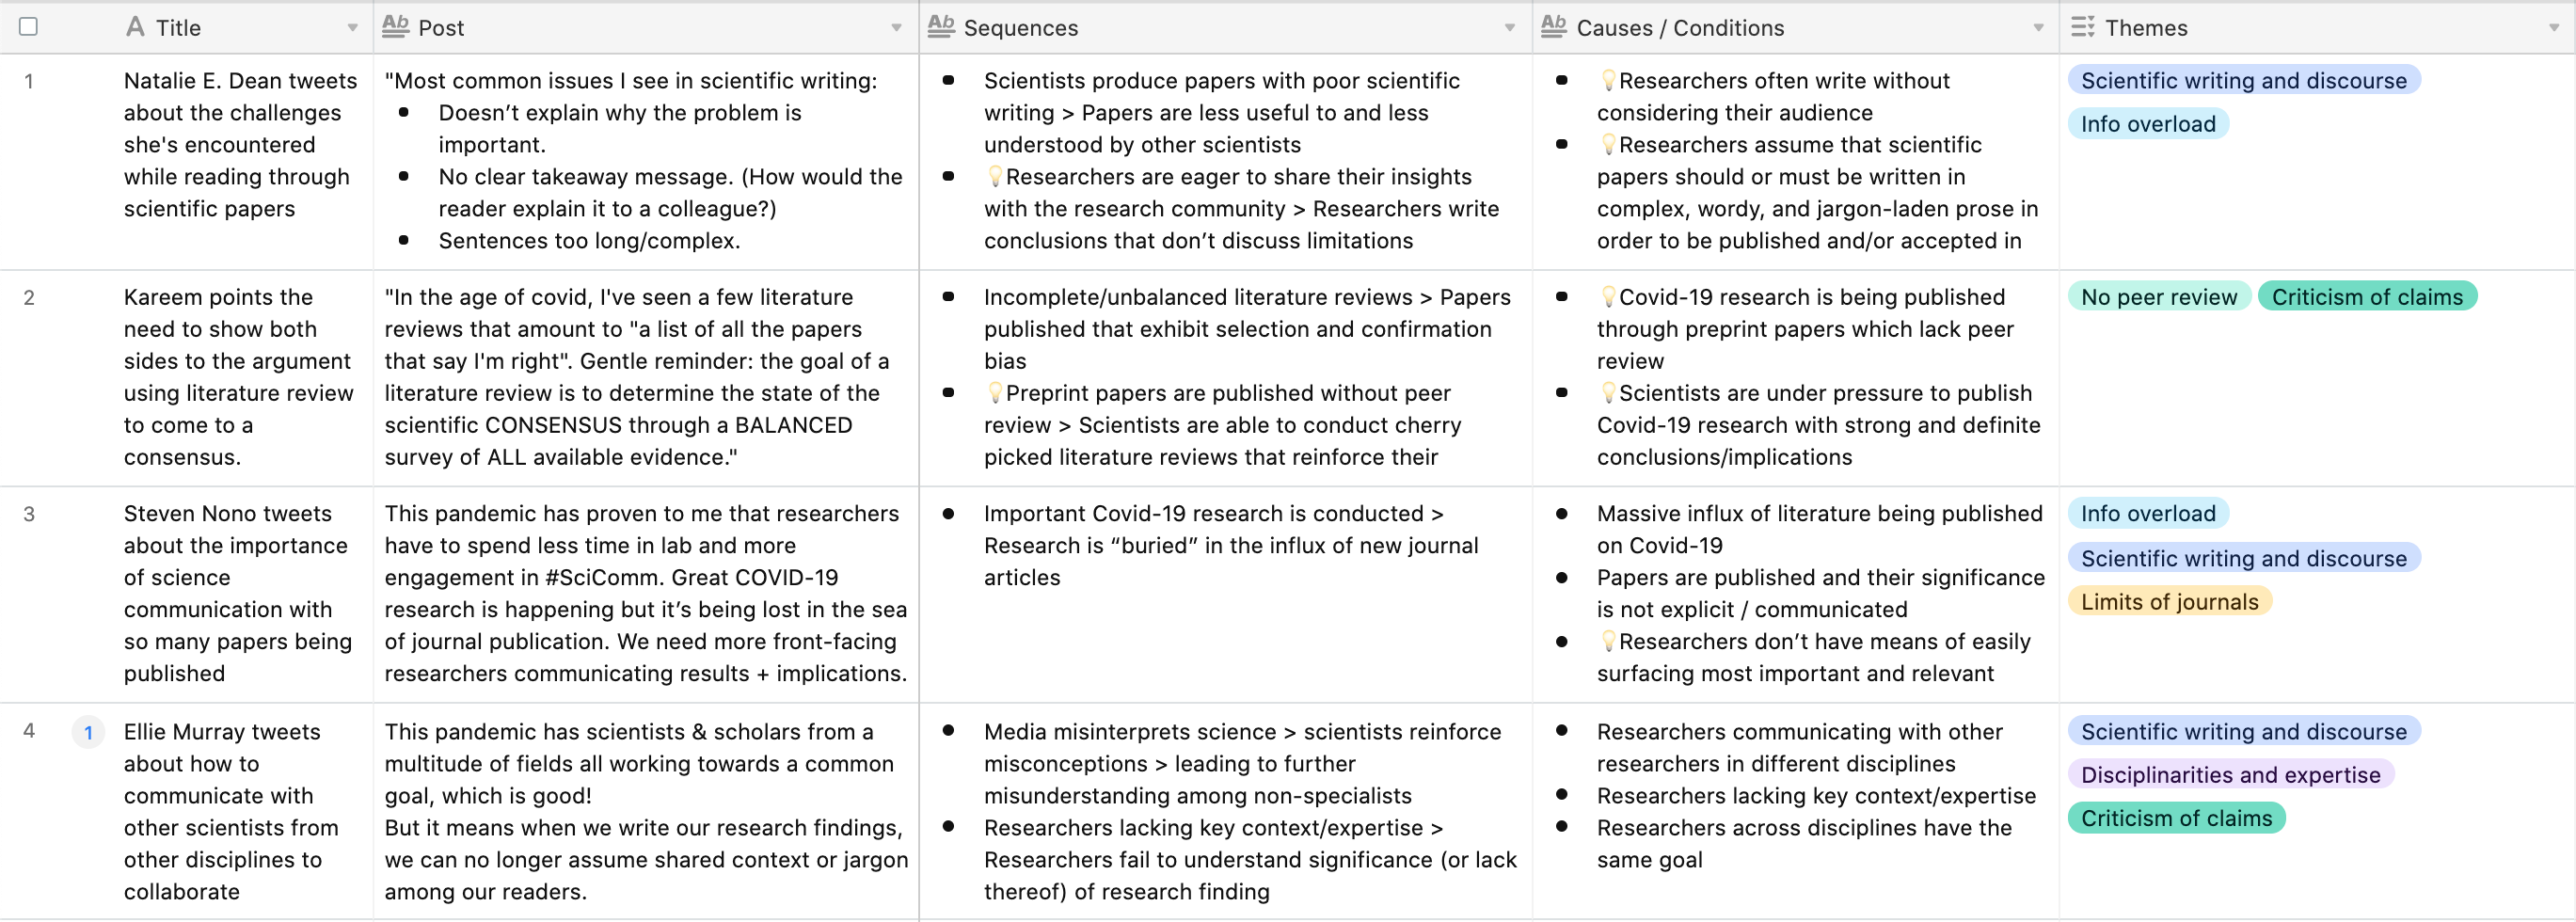
\includegraphics[width=1\textwidth]{Pictures/Airtable.png}
  \caption{Our open coding of tweets using Airtable}
  \Description{Our open coding of tweets using Airtable}
  \label{airtable}
\end{figure}

%Figure: Affinity diagram

\section{Analysis and Results}
\label{Analysis_and_Results}
Online communities of researchers emerge out of a need to collectively summarize, share, and discuss recently published studies (i.e., to quickly and efficiently share scientific knowledge). This section focuses particularly on the inefficiencies and unsuitability of current information organization and filtration mechanisms of these platforms for the scientific community. We also highlight the consequences of not having an appropriate infrastructure in place for scientists during the COVID-19 pandemic and the necessity for it.

%TODO: Add more tweets for this subsection
One example of Twitter being used to summarize and disseminate recent scientific research can be seen in a tweet by Professor Francois Balloux ($3,000$ RT, $5,100$ L):
``Over the last weeks, a substantial amount of new evidence has become available about immunity to \#SARSCoV2. This information can be difficult to process and integrate. As such I felt it may be helpful to write a thread to summarise the information and provide some context ($1$/$13$) \citep{balloux_2020}. ''Understanding copious amounts of new literature regarding COVID-19 literature is timeconsuming and tiresome to do by oneself.

While Balloux acknowledges these difficulties, he also provides insight into an important solution - the power of crowds. By summarizing the literature and sharing it with others to more efficiently learn the novelty of the findings, he has saved other researchers more time than he spent in his efforts. 

Much of the struggle COVID-19 researchers are facing with effectively sharing knowledge could be alleviated with more awareness of the issues. Through our analysis of tweets and recently published articles, we identified the following themes of challenges to the large-scale scientific knowledge sharing during the COVID-19 pandemic:

\begin{itemize}
    \item Shortcomings of scientific knowledge sharing on Twitter;
    \item Preserving quality of evaluation while increasing speed;
    \item Difficulties in efficiently informing research community about inappropriate results/interpretations in papers;
    \item Reliance on bibliometrics and altmetrics;
    \item Repetition in Published Papers;
    \item Rigidity of papers;
    \item Difficulties in multidisciplinary research.
\end{itemize}

Throughout the rest of this section we will discuss our analysis of each of these challenges in details. We refer to all authors of tweets by the specific profile name they used on Twitter at the time we collected their tweet. Additionally, we will be including the number of retweets(RT) and likes(L) as part of tweet descriptions. 

\subsection{Shortcomings of Scientific Knowledge Sharing on Twitter}
\label{Shortcomings of Scientific Knowledge Sharing on Twitter}

In lack of a platform tailored for and populated by scientists for collective knowledge sharing, researchers have turned to Twitter as a very popular social media platform for research communication. Researchers have turned to Twitter as a very popular social media platform for research communication \citep{collins2016scientists, ke2017systematic, van2011scientists}. However, this platform lacks key design affordances needed to address the particular needs of users engaged in scientific knowledge sharing. As evinced by Professor Francois Balloux's tweet in 
% \autoref{balloux_tweet}
, Twitter is used by researchers to quickly and efficiently share knowledge, but the dissemination of misinformation and an experience that is not tailored to research communication has left researchers using the platform looking for more support.
PTPeters tweeted ($1$ RT, $1$ L) ``The word limit, and fleeting nature of Tweets, makes this format best for a simple IT KSM: Knowledge Sharing Network. ... Twitter is not good format for debate... \citep{Peters2020twitter}.''

\citet{lacassin2020rapid} call the reliability and legitimacy of knowledge sharing on Twitter into question, due to the lack of peer-review of the content. Additionally, they claim that some scientists may be reluctant to share novel findings or knowledge on Twitter because there is a chance of publishing the data or analysis by other researchers rather than the original author. It can be dangerous to both the public and research community when unreliable content is widely disseminated on Twitter. Dr. Krutika Kuppalli describes this situation in \autoref{kuppalli_tweet} referring to a tweet made by Michael Levitt, with $2K$ RT, $4.5K$ L.

\begin{figure}
  
\includegraphics[width=0.6\textwidth]{Pictures/kuppalli_tweet.png}
  \caption{Twitter used to disseminate inaccurate information by academics with institutional credibility \citep{kuppalli2020twitter}.}
  \Description{Twitter used to disseminate inaccurate information by academics with institutional credibility \citep{kuppalli2020twitter}.}
  \label{kuppalli_tweet}
\end{figure}

\citet{pershad2018social} discuss the drawbacks of knowledge sharing on Twitter in medical sciences. One issue is that the limited number of characters in tweets restrains researchers to briefly convey sophisticated research, which may result in miscommunications and negatively impact scientific communication. The second problem is the time required to go through all tweets to self-judge and filter the necessary information. For instance, $80$\% of tweets from reliable professionals are posted during the workday, from $9$ a.m. to $5$ p.m. that may deprive health care workers to allocate their time to patient care routines.

Researchers are using Twitter to communicate science. While some take their papers to social media to share, others use the platform to actively challenge studies that they found misleading, as an unofficial form of quality control \citep{Brainard2020drowning}. In a conversation among researchers on Twitter, the context of the conversation can get confusing. A researcher may have a diverse set of followers from many backgrounds: other researchers (possibly from different disciplines), laypeople, politicians, etc. This can have negative ramifications on how a message is framed and received, since different audiences can react differently to the same message. Kareem Carr tweeted ($156$ RT, $486$ L) ``One big problem is there are at least four possible ways for a scientist to have a conversation on Twitter...Talking to other scientists as a scientist...Talking to other scientists as a member of the public...Talking to the public as a scientist...Talking to the public as a member of the public...These conversations are happening all at once and it can change from sentence to sentence. Scientists are generally not good about specifying the role we're playing in public discussions. This can lead to terrible fights \citep{carr2020twitter}.'' 


\subsection{Preserving Quality of Evaluation While Increasing Speed}
\label{Preserving quality of evaluation while increasing speed}

Rapid dissemination of the COVID-19 research findings is important to facilitate the acceleration of the research. Dissemination of fast and rapidly reviewed papers makes researchers self-judge and screen most of the studies on their own, which is extremely time-consuming. While fast dissemination of factual information is beneficial, misinformation can grow fear and panic or cause lethal movements in society \citep{reuters2020speed}. \citet{palayew2020pandemic} stresses the importance and the need for novel solutions to guarantee sustainable trust in the large-scale scientific publishing process during a pandemic. They conducted single-query searches on PubMed and analyzed data for COVID-19 and Ebola-related papers. The results showed that COVID-19 publications had a median acceptance time of 6 days, while it was about 15 days for Ebola. The fast dissemination of information is needed to keep up with a global pandemic but has cast doubt on the quality of publications and the probability of misinformation \citep{palayew2020pandemic}. Some medical journals have drastically reduced publication time \citep{horbach2020pandemic, Kupferschmidt2020culture}. Peer-review delay has been reduced by $49$\%, or $57$ days on average (even higher for some journals like Archives of Virology) \citep{horbach2020pandemic}. Fourteen medical journals that published most COVID-19 papers reduced the average time taken from submission to publication to about $60$ days \citep{Brainard2020drowning}, which may adversely affect the quality of published papers.

Lonni Besançon investigated $12,682$ publications related to COVID-19 on PubMed. Their study revealed that about $8$\% of papers were published in the day that they were submitted. What can be inferred is that the peer-review process might have been rushed for some papers. Editorial conflicts of interest were recognized in $43$\% of these papers. Such a short acceptance interval raises concerns about the integrity and clearness of the peer-review process \citep{besanccon2020open}. Some concerns regarding quick peer-review surround the ethics of research being done. Mamas tweeted ($74$ RT, $145$ L): ``Pandemic vs paperdemic, the risks of speed science and research ethics as exemplified by \#covid19 Sometimes we take at face value the honesty of researchers and veracity of data \citep{Mamas2020twitter}.'' Mamas' concerns are noteworthy given recent scandals surrounding data that could have cost lives, namely Surgisphere's mishandling of Hydroxychloroquine data \citep{servick2020pandemic}. Sapan Desai, the founder of Surgisphere who has published two papers in the most reputable medical journals, is currently being sued in two different medical mal-practiced cases and had incentive to promote work using data from his company, and yet the Lancet and New England Journal of Medicine both published his work in fields completely unrelateed from his expertise, largely due to a lack of adequate peer-review \citep{piller2020s}.

Falsified data and misleading findings in publications may also stain the reputation of journals and decrease public trust in scientific findings. Gregory Makles tweeted ($0$ RT, $0$ L): ``NEJM is suddenly reliable again? Have they investigated their latest peer review incredible failure? \citep{Makles2020twitter}." 

Speedy peer-review is not the only gateway for improper research to disseminate throughout the scientific community. Preprints, who publish work with no peer-review process also pose a threat.
Block tweeted ($0$ RT, $0$ L): ``...I'm seeing a ton of COVID-19 pre-print research coming out, though that poses issues of its own because of lack of peer review \citet{Block2020twitter}.'' 
Preprints have certainly been a useful resource for scientists to communicate with one another efficiently, but at what cost?


\subsection{Difficulties in Efficiently Informing Research Community About Inappropriate Results/interpretations in Papers}
\label{Difficulties in efficiently informing research community about inappropriate results/interpretations in papers}

Researchers have expressed concerns about the lack of an efficient mechanism to communicate their criticisms. After analyzing recent studies, they lack a unified platform to document their criticisms. Other researchers who come across the same studies may not be aware of those criticisms if they do not have contact with previous readers or forgot what has been critiqued. 

We have noticed many instances that researchers express their frustrations in informing the research community when they identify issues in analysis, methods, results, or interpretations reported in a paper. An example of researchers using Tweets to inform the research community about retracting a paper is shown in \autoref{Elisabeth_Tweet}. Other examples of advocating on social media for retraction on Twitter is shown in \autoref{Retraction_Tweets}. The use of Twitter for science communication has been very valuable, however for reasons we discuss in \autoref{Shortcomings of Scientific Knowledge Sharing on Twitter}, system design tailored to science communication are needed.

In a recent study, it was found that the researchers' followers on Twitter are relatively low and only $25$\% of researchers have more than $429$ followers\citep{costas2020comparison}. Another study discusses that nearly $40$\% of scientists' followers are nonscholars \citep{cote2018scientists}. 
Also, it was shown that only $1.1$\% of Web of Science researchers in the field of biomedical and health sciences use twitter. And the use of twitter by scholars is mostly ($40$\%) confined to the USA and the UK \citep{costas2020large}.

\begin{figure}
  
\includegraphics[width=0.5\textwidth]{Pictures/elisabeth_tweet.png}
  \caption{An example of researchers using blog posts, Tweets, and any medium they can to inform the research community about retracting a paper \citep{Elisabeth2010twitter}}
  \Description{An example of researchers using blog posts, Tweets, and any medium they can to inform the research community about retracting a paper.}
  \label{Elisabeth_Tweet}
\end{figure}


\begin{figure}
\centering
\parbox{5cm}{

\includegraphics[width=0.4\textwidth]{Pictures/retraction watch tweet.png}
}
\qquad
\begin{minipage}{5cm}

\includegraphics[width=1.2\textwidth]{Pictures/carlos tweet.png}
\end{minipage}
 \caption{Examples of advocating for retraction on Twitter \citep{Retract2010twitter, Carlos2020twitter}}
 \Description{Examples of advocating for retraction on Twitter.}
 \label{Retraction_Tweets}
\end{figure}


\subsection{Reliance on Bibliometrics and Altmetrics Exacerbates the Issue}
\label{Reliance on bibliometrics and altmetrics exacerbates the issue}

Bibliometrics is a set of methods for estimating scholarly impact which might generate conflicts and concerns \cite{roemer2012bibliometrics}. Internet-based impact metrics known as alternative metrics or altmetrics were proposed to mitigate those problems. 
There is an ongoing challenge to find and develop new methods for tracking scholarly impact \cite{roemer2012bibliometrics}. Merely relying on citation count as a metric to measure the \textit{quality} of research papers has exacerbated the difficulties bound up with efficiently informing the research community of inappropriate results and/or interpretations.

It is shown that the number of citation and publications are not a reliable gauge for scholars' talent and scientific merits \citep{ruocco2017bibliometric}. NatureNews tweeted ($0$ RT, $0$ L): ``...Bibliometrics alone clearly do not offer a reliable way to gauge the quality of research \citep{Nature2010twitter}.'' Joe Kraus tweeted ($0$ RT, $0$ L): ``...Citation data does not provide reliable evidence of quality of research \citep{Kraus2013twitter}.''
% Explanation of method. Make more clear. Should example at end be removed? 
This heuristic can be misleading, especially, in case of retractions. We observed that retracted papers continue to receive citations. As an example, on 3/20/2020, a paper titled, ``Hydroxychloroquine and azithromycin as a treatment of COVID-19: results of an open-label non-randomized clinical trial'' was published by International Journal of Antimicrobial Agents \citep{gautret2020hydroxychloroquine}. The manuscript appeared on medRxiv on 3/16/2020. It was also submitted to the International Journal of Antimicrobial Agents on 3/16/2020. The paper was accepted for publication by the journal on 3/17/2020, and was published on 3/20/2020. This paper raised many concerns by multiple scientists on Twitter and ten days after publication, on 3/30/2020, another article titled, ``A Rush to Judgment? Rapid Reporting and Dissemination of Results and Its Consequences Regarding the Use of Hydroxychloroquine for COVID-19'' \citep{kim2020rush} was published by Annals of Internal Medicine, retracting \citet{gautret2020hydroxychloroquine} and pointing out various flaws in it. However, as of 09/02/2020, while \citet{gautret2020hydroxychloroquine} has received $2,304$ citations on Google Scholar, \citet{kim2020rush} has received only $97$. We hypothesized that most of the papers citing \citet{gautret2020hydroxychloroquine} may have criticized or retracted it. However, reviewing a random sample of $100$ papers out of the $2,304$ that were citing the study, showed that $82$ out of $100$ papers were using the results or reporting follow-up studies, which indicates inefficiency of:
\begin{itemize}
   \item Evaluation of publications merely based on their number of citations;
   \item Informing the research community about inappropriate results/interpretations in papers.
\end{itemize}
As another example, a paper titled ``Cardiovascular Disease, Drug Therapy, and Mortality in Covid-19'' was retracted on 4/6/2020 and had $358$ citations however by 9/13/2020 the number of citation had reached $452$. We hypothesized that it might be because the upcoming papers are retracting the original paper. We randomly went through $25$ of those papers and to our surprise, $18$ of those papers were really exploiting the findings of the retracted paper. 
To be able to compare the results we checked a third paper titled ``SARS-CoV-2 infects T lymphocytes through its spike protein-mediated membrane fusion'' was published in Nature Cellular \& Molecular Immunology on $4/7/2020$ and retracted about three months later on $7/10/2020$ \citep{wang2020sars}. By $9/13/2020$ this paper had $152$ citations. We randomly picked $10$ out of $40$ papers citing that paper, which were published after the retraction date. We observed that only one paper was retracting the original paper. This might be due to prolonged delay before retracting.


The problem with retracted papers and how often they are cited is summarized in a tweet by Andrew R. Timming ($34$ RT, $334$ L): ``Why the h-index is a poor performance metric: I could write a bunch of egregiously bad papers and everyone would cite them by pointing out all the flaws. Plus, it punishes single authored papers and artificially inflates the worth of co-authored ones. Am I wrong? \citep{timming_2020}''


%TKTK We have to do the same thing for other retracted papers.

% \subsection{Inefficacy of NLP-based Research Summarization Tools}
% \label{Inefficacy_of_NLP_based_Research_Summarization_Tools}

%and progress in research. 
%to mitigate the previous three issues, COVID-19 researchers have created 

% \subsection{Infrastructure: Inefficient Organization/filtration of Information}
% \label{Infrastructure: Inefficient organization/filtration of information}


\subsection{Repetition in Published Papers}
\label{Repetition in Published Papers}
%Need more tweets
To allow researchers to keep up with the massive and rapid dissemination of academic papers, it is important that the redundancy of content is as minimal as possible. With no great way to signal to an entire community what has already been done, we are in danger of wasting resources on what is already known (see \autoref{philippe_tweet} and \autoref{konig_tweet}). Take the hydroxychloroquine controversy where an excess of evidence came out against its efficacy, possibly wasting valuable time, energy and risk in the process. In \autoref{Barbasi_Tweet} Barb\'asi tweets about the issue of redundancy as it pertains to active trials regarding hydroxychloroquine, stating that there was a whopping total of 77 active trials within the previous day. Barb\'asi goes as far as to place the blame on "...lock[ing] out the science...", and letting twitter drive research directions (see \autoref{Shortcomings of Scientific Knowledge Sharing on Twitter} for more analysis on why twitter is not the optimal place for scientific dissemination). 

Richard Poynder tweeted: ``The number of publications related to COVID‐19 is growing exponentially. Many articles are being hastily and non-critically published, contain repetitive or inaccurate information, illogical and non-evidence based recommendations, and are highly biased \citep{poynder2020twitter}($5$ RT, $12$ L)." 


Dmitri Zaitsev shared their hopes for reducing redundancy and the problems it creates: ``When this pandemic subsides we could use this situation as a motive to reduce redundancy in publication, to modernize the way data is presented, and to avoid the same issues when the new pandemic arrives.- Any details about how that would happen? :) \citep{zaitsev2020twitter}($0$ RT, $1$ L).''

\begin{figure}
  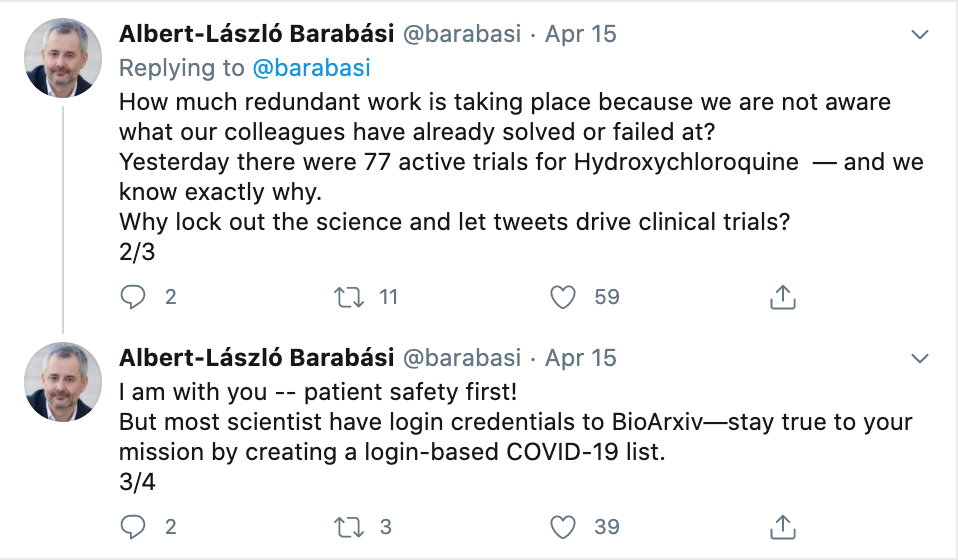
\includegraphics[width=0.6\textwidth]{Pictures/barabasi tweet.png}
  \caption{Repetition in published papers \citep{Barbasi2020twitter}}
  \Description{Repetition in published papers}
  \label{Barbasi_Tweet}
\end{figure}

\begin{figure}
  
\includegraphics[width=0.6\textwidth]{Pictures/philippe_tweet.png}
  \caption{Repetition in published papers \citep{Philippe2020twitter}}
  \Description{Repetition in published papers}
  \label{philippe_tweet}
\end{figure}

\begin{figure}
  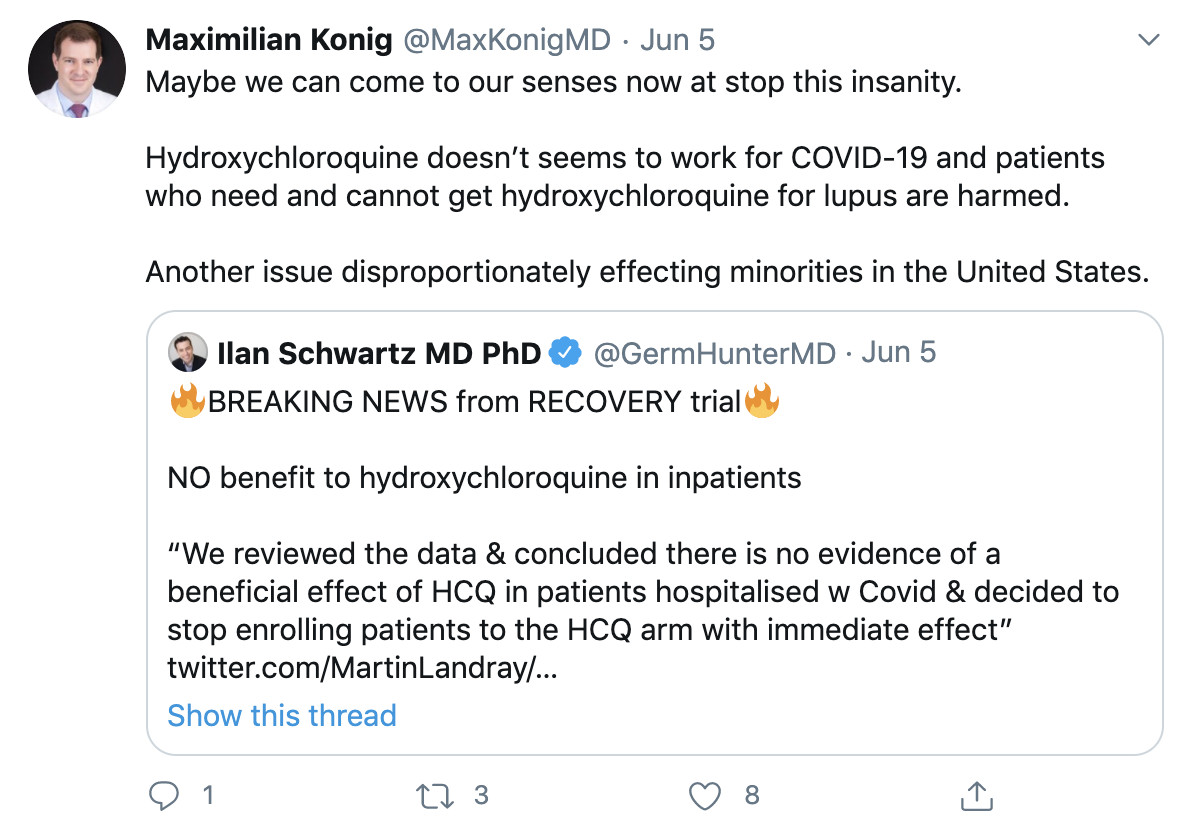
\includegraphics[width=0.6\textwidth]{Pictures/konig tweet.png}
  \caption{Repetition in published papers \citep{Konig2020twitter}}
  \Description{Repetition in published papers}
  \label{konig_tweet}
\end{figure}

\subsection{Rigidity of Papers}
\label{Rigidity_of_Papers}

When a paper is published, its content stays static. 
Review papers of the publications of the previous day or week have gained significant attention, but they often miss some of the main points or misinterpret findings. As new investigations are made, there is no way to update these papers. Egon Willigh tweeted ``I am really frustrated with the fact that our publications are static objects. why can't we improve them over time?... \citep{Will2018twitter}.'' 

This may be especially problematic when the number of citations is considered to be the primary metric to assess the quality of a publication and whether to pay attention to it. It would take a fair amount of time for new publications to get a comparable number of citations (Mathew's effect \citep{beel2009google}) to grab attention and make the outdated papers obsolete, similar to the problems discussed in \autoref{Reliance on bibliometrics and altmetrics exacerbates the issue}. George Musser tweeted ($2400$ RT, $3200$ L): ``Google Scholar seems to be altering scholarly citation patterns. Citations are getting more concentrated: the same few papers get cited over and over, @jevinwest has found. People lazily cite whatever papers the search engine ranks highly \citep{Musser2019twitter}.''

 Jeffrey Barrett tweeted about desiring the capability of editing papers that have content that is redundant and not relevant in the near future ($4$ RT, $36$ L): ``I don't know who needs to hear this, but if you're writing a paper about Covid-19, just delete the sentence that states there is a pandemic and provides the current (already out of date) estimate of the number of global cases and deaths. Just. Delete. It. \citep{Barrett2010twitter}." 
 His sentiment echoes the claims from \autoref{Repetition in Published Papers}, that too much space in COVID-19 literature is used to repeat the same things to the same same audience. 
 
 To mitigate this problem a system called Manubot has been suggested.  Manubot is an open collaborative authoring platform providing handy version control and multiple access levels.
 Casey Greene tweeted, asking about its usage ($1$ RT, $13$ L): ``What if you're writing a collaborative review paper using manubot, and you use its capabilities to update from external data sources each night? \citep{Greene2020twitter}."  While Manubot works to alleviate some of the problems, using it requires some computational skils (e.g version control workflows and GitHub). Also, discussions between writers are not tracked using Git \citep{himmelstein2019open}. As a result, collaborative authoring in many disciplines including medical science and epidemiology might be not very efficient using the platform \citep{himmelstein2019open}.


\subsection{Difficulties in Multidisciplinary Research}
\label{Difficulties in Multidisciplinary Research}
 
Large-scale collaboration across different disciplines presents obstacles in reaching shared research goals due to differences in terminology and context within each discipline. Many researchers have taken to Twitter, open conversations about this insufficiency.

Ellie Murray tweets about how to communicate with other scientists from other disciplines to collaborate ($58$ RT, $221$ L): 
``This pandemic has scientists \& scholars from a multitude of fields all working towards a common goal, which is good! But it means when we write our research findings, we can no longer assume shared context or jargon among our readers \citep{Murray2020twitter}.'' 

``There's been a fair amount of discussion of the dangers of pre-prints being misinterpreted by the public or journalists. But, we don't talk about a potentially more dangerous issue: scientists \& scholars in other disciplines getting the wrong message b/c they lack key context \citep{Murray2020jargon}."

Murray continues in another tweet ($2$ RT, $36$ L): 
``Second, since combating the pandemic is our shared goal, any failure to communicate between scientists \& scholars creates a barrier to achieving that goal, and thus has a cost in human lives lost \citep{Murray2020pandemic}." 

Another tweet, by Dr. Angela Rasmussen, discusses the difficulty of communicating across disciplines because of different definitions and contexts to terms used in different disciplines ($9$ RT, $53$ L): 
``I think the real problem has been communication across disciplines. The terminology is confusing and means different things to different people, which is why I agree with \@SaskiaPopescu that we need to reconsider the language we use to discuss airborne' transmission \citep{Rasmussen2020twitter}.''


\section{Discussion and Design Implications}
\label{Discussion_and_Design_Implications}

% \subsection{How to cope with the massive influx of COVID-19 papers?}
We found that researchers are having a difficult time keeping up with the massive influx of papers. This is due in part to the use of inefficient methods of organization and filtration of information that do not work at scale. Cognitive overload is being imposed on COVID-19 researchers as they struggle to stay aware of what has been studied.

Readers familiar with Natural Language Processing (NLP) may feel that the question of its efficiency in facilitating scientific knowledge summarization must be addressed. Many applications using NLP algorithms have been developed to summarize the newly published papers and reduce the overload on scientists who must review hundreds of newly published papers every day. However, researchers have raised concerns over NLP-based tools promoting retracted papers or papers with overstated findings \citep{Brainard2020drowning}. One reason for this issue is the fact that the content of about $20\%$ of subscribers-only journals papers is not free to download (which has a forecasted trend of a $50\%$ increase) and therefore, cannot be reviewed by NLP-based tools \citep{Brainard2020drowning}. Even among  free publications, many of their papers are in a PDF format, which are not considered to be FAIR (Findable, Accessible, Interoperable, Reusable) and therefore cannot be processed by NLP algorithms \citep{oelen2020generate}. To train machine learning models, researchers rely on preprint databases such as \url{arXiv.org} to be able to retrieve the content of a large number of papers for free \citep{Brainard2020drowning}.

In addition, reviewing the papers can be its own challenge. Scientific jargon is often complex and difficult to understand even by human standards. The terminology found in peer-reviewed literature is not always present in the mainstream text where the model training is performed. This problem is more common when the literature is domain-specific (outside of the training domain). This is present in the CORD-19 dataset (and others), leading to adverse effects on the fine tuning of the text summarization models \citep{kieuvongngam2020automatic}. Some scholars also doubt the efficacy of automated procedures to help the research community. In our informal interviews with COVID-19 PIs, two of them told us ``automated text summarization is very helpful for use-cases like distilling product reviews on amazon, but research papers are totally different. If understanding the analysis or findings in research studies was that easy, our undergraduate students would be able to do it and we would not need to spend so much time reviewing papers on our own.''

COVID-19 researchers' need for a faster mechanism to learn about new studies on one hand, and their frustration with the NLP-based text summarization services, on the other hand, necessitates design and development of an online crowdsourced research hub, where researchers collaboratively summarize newly published literature and continuously update it as new findings are published. Every day COVID-19 researchers and their students study and summarize newly published research papers. They present their summaries in focus groups, classes, and journal clubs to help each other cope with the accelerated rate of publications. For the same reason, some research groups have also focused on publishing review papers of studies published in the past few days to help a larger community of researchers. However, focus groups and journal clubs are only helpful for small groups of people. Review papers are also rigid (as discussed in \autoref{Rigidity_of_Papers}) and any misinterpretation or missing findings of a study would not be corrected until new review papers make the old ones completely obsolete. The time and energy used by the existing research community could be more efficiently utilized if an online crowdsourcing research hub existed which would enable researchers to collaboratively summarize, discuss, comment, and criticize research publications.

In the remainder of this section, we discuss and ideate the necessary features of such a research hub to mitigate the issues discussed in the analysis and results section. We follow the same order of classifications of difficulties based on the themes identified from the analyzed tweets.

\subsection{Difficulties in efficiently informing research community about inappropriate results/interpretations in papers}
\label{Discussion_Difficulties_in_efficiently_informing_research_community}
Our analysis of tweets indicates that many COVID-19 researchers experience difficulties to find a tribune to let other researchers hear their voice. They have expressed a need for a large-scale online research hub only for certified researchers, where they can easily access:
\begin{itemize}
   \item Each other’s names and validated credentials;
   \item Published papers with their number of citations;
   \item Comments about each publication and related discussions;
   \item Classified questions and answers about each topic;
   \item Direct contact channel to other researchers for follow-up questions/comments.
\end{itemize}

\subsection{Reliance on bibliometrics and altmetrics}
We found many tweets indicating the researchers’ reliance on citation count to assess the quality of research papers has mislead many, especially in the case of retracted papers. While algorithms such as PageRank \citep{page1999pagerank} have been proven helpful for website searching, similar citation-based ranking does not necessarily guarantee the quality of research papers. While altmetrics also consider mentions of a paper on tweets, blogposts, and other online social networks, it is still insufficient. A mere citation does not indicate anything about the quality of a study. In the research context, a citation should be assigned a positive, neutral, or negative weight. Then a weighted summation of the citations could be produced and it would be a more accurate metric for evaluation of research papers.
\begin{itemize}
   \item \textbf{Positive}: if a study is cited to be admired/replicated/continued/rederived in another paper.
   \item \textbf{Neutral}: if a study is cited to be reviewed/meta-analyzed/classified in another paper.
   \item \textbf{Negative}: if a study is cited to be retracted/contradicted/corrected in another paper.
\end{itemize}

\subsection{Difficulties in multidisciplinary research}
The COVID-19 pandemic has made the need for multidisciplinary research more prominent than ever. However, COVID-19 researchers’ tweets indicate that they need a more efficient communication method between researchers from different disciplines. They need a common ground around a shared set of vocabulary that can be easily deciphered by any researcher, regardless of their discipline and specialty area. To fulfill this objective the large-scale online research hub should provide a new search UI to researchers where they can easily find the term/concept they need to understand and facilitate back-tracking prerequisite concepts to be learned to understand the searched query.

Conventionally, scientific jargon or words are highly interdependent to each other where understanding one requires understanding others and to understand the others, one should read a graduate level textbook. This makes building a common ground between researchers extremely difficult. To solve this issue, a collaborative prerequisite linking mechanism is necessary where researchers link every concept/term/jargon to its prerequisites and expand upon them. This should be an asynchronous collaborative process because the scale of the terminology in different disciplines is growing fast and providing data to such a search tool requires crowdsourcing and collaboration between many scientists and possibly their students. The tool should enable researchers to start from a term/concept and back-track the prerequisite knowledge required to understand that term/concept recursively. Compared to the conventional method of studying a textbook to learn a new field’s jargon, this tool enables researchers to only focus on the concepts/terms necessary to efficiently learn what they need without getting distracted by other concepts or discussions around them.


\section{Conclusion}
\label{Conclusion}
































%%
%% The next two lines define the bibliography style to be used, and
%% the bibliography file.
\bibliographystyle{ACM-Reference-Format}
\bibliography{Iman_Cognitive_Psychology_Learning}

%%
%% If your work has an appendix, this is the place to put it.
\appendix
\section{Tweets}

\begin{figure}
  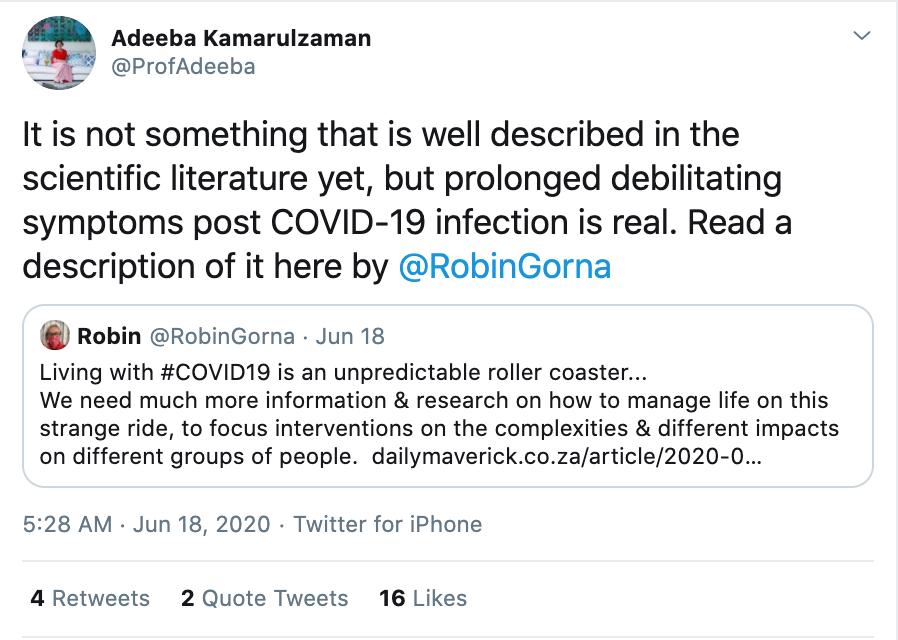
\includegraphics[width=0.5\textwidth]{Pictures/Appendix_Tweets/adeeba kamarulzaman tweet.png}
  \caption{Adeeba Kamarulzaman tweets about COVID-19 findings that are not yet widely talked about in scientific literature}
  \Description{Adeeba Kamarulzaman tweets about COVID-19 findings that are not yet widely talked about in scientific literature}
  \label{adeeba_kamarulzaman_tweet}
\end{figure}

\begin{figure}
  
\includegraphics[width=0.5\textwidth]{Pictures/Appendix_Tweets/alice sim tweet.png}
  \caption{Alice Sim tweets about fueling the infodemic with misinterpreted terminology}
  \Description{Alice Sim tweets about fueling the infodemic with misinterpreted terminology}
  \label{alice_sim_tweet}
\end{figure}

\begin{figure}
  
\includegraphics[width=0.5\textwidth]{Pictures/Appendix_Tweets/andy slavitt tweet.png}
  \caption{Andy Slavitt tweets about the variety of sources of information and the public being unaware of the differences}
  \Description{Andy Slavitt tweets about the variety of sources of information and the public being unaware of the differences}
  \label{andy_slavitt_tweet}
\end{figure}

\begin{figure}
  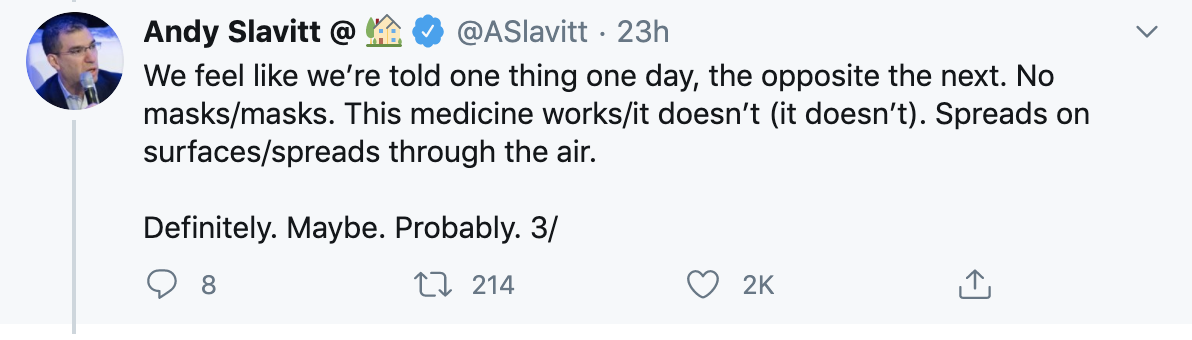
\includegraphics[width=0.5\textwidth]{Pictures/Appendix_Tweets/andy slavitt tweet2.png}
  \caption{Andy Slavitt tweets about confusion over scientists advice}
  \Description{Andy Slavitt tweets about confusion over scientists advice}
  \label{andy_slavitt_tweet2}
\end{figure}

\begin{figure}
  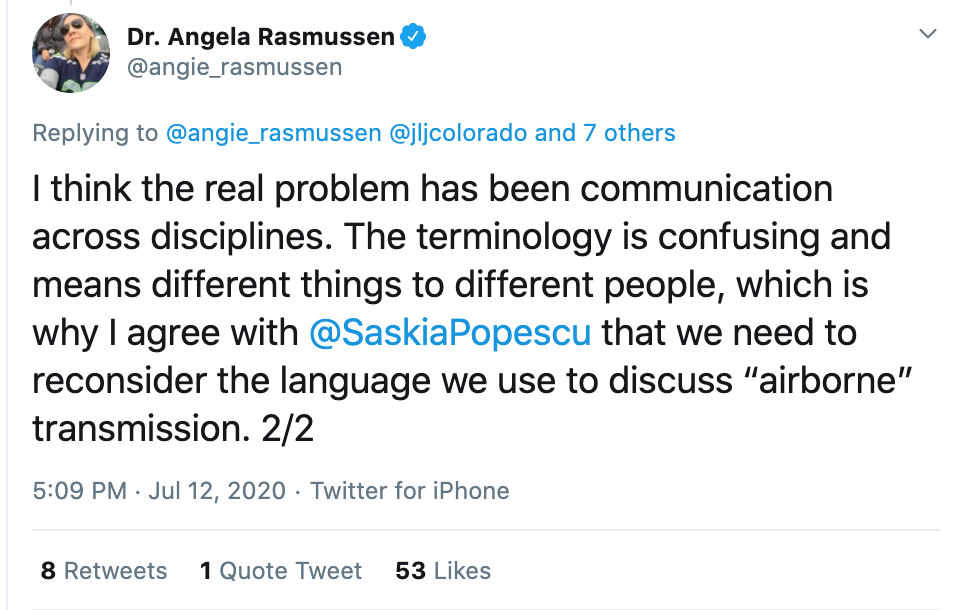
\includegraphics[width=0.5\textwidth]{Pictures/Appendix_Tweets/angela rasmussen tweet.png}
  \caption{Dr.Angela Rasmussen tweets about the miscommunication across disciplines}
  \Description{Dr.Angela Rasmussen tweets about the miscommunication across disciplines}
  \label{angela_rasmussen_tweet}
\end{figure}

\begin{figure}
  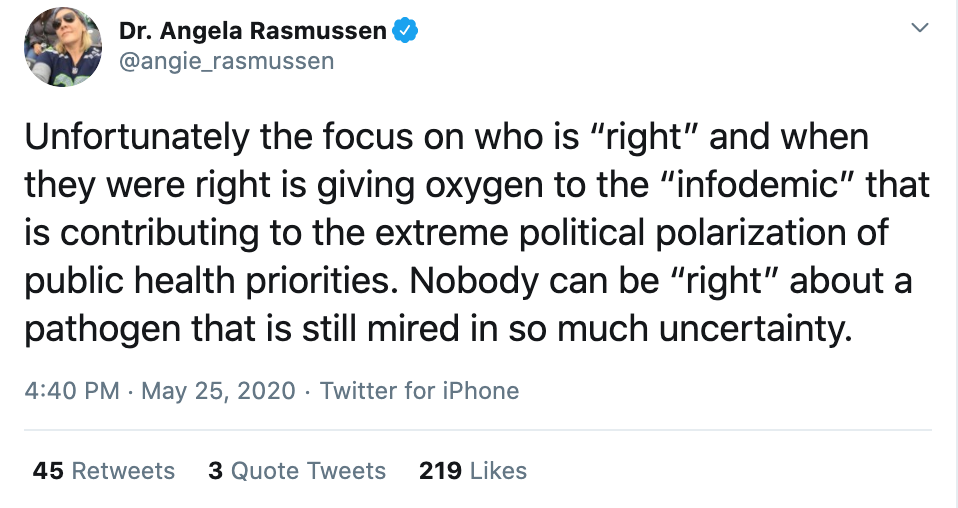
\includegraphics[width=0.5\textwidth]{Pictures/Appendix_Tweets/angela rasmussen tweet2.png}
  \caption{Dr.Angela Rasmussen tweets about the focus on validity of statements}
  \Description{Dr.Angela Rasmussen tweets about the focus on validity of statements}
  \label{angela_rasmussen_tweet2}
\end{figure}

\begin{figure}
  
\includegraphics[width=0.5\textwidth]{Pictures/Appendix_Tweets/angela rasmussen tweet3.png}
  \caption{Dr.Angela Rasmussen tweets how painting WHO as the enemy is counterproductive in terms of coming to a consensus}
  \Description{Dr.Angela Rasmussen tweets how painting WHO as the enemy is counterproductive in terms of coming to a consensus}
  \label{angela_rasmussen_tweet3}
\end{figure}

\begin{figure}
  
\includegraphics[width=0.5\textwidth]{Pictures/Appendix_Tweets/angela rasmussen tweet4.png}
  \caption{Dr.Angela Rasmussen tweets about the harm of others not sharing data and being unable to make her own analyses}
  \Description{Dr.Angela Rasmussen tweets about the harm of others not sharing data and being unable to make her own analyses}
  \label{angela_rasmussen_tweet4}
\end{figure}

\begin{figure}
  
\includegraphics[width=0.5\textwidth]{Pictures/Appendix_Tweets/austin wright tweet.png}
  \caption{Austin L. Wright tweets about using a variety of resources for finding papers}
  \Description{Austin L. Wright tweets about using a variety of resources for finding papers}
  \label{austin_wright_tweet}
\end{figure}

\begin{figure}
  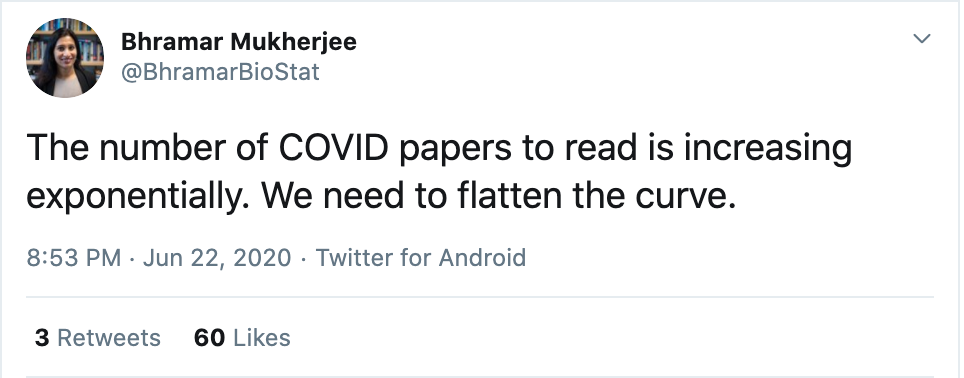
\includegraphics[width=0.5\textwidth]{Pictures/Appendix_Tweets/bhramar mukherjee tweet.png}
  \caption{Bhramar Mukherjee tweets about the increasing number of papers}
  \Description{Bhramar Mukherjee tweets about the increasing number of papers}
  \label{bhramar_mukherjee_tweet}
\end{figure}

\begin{figure}
  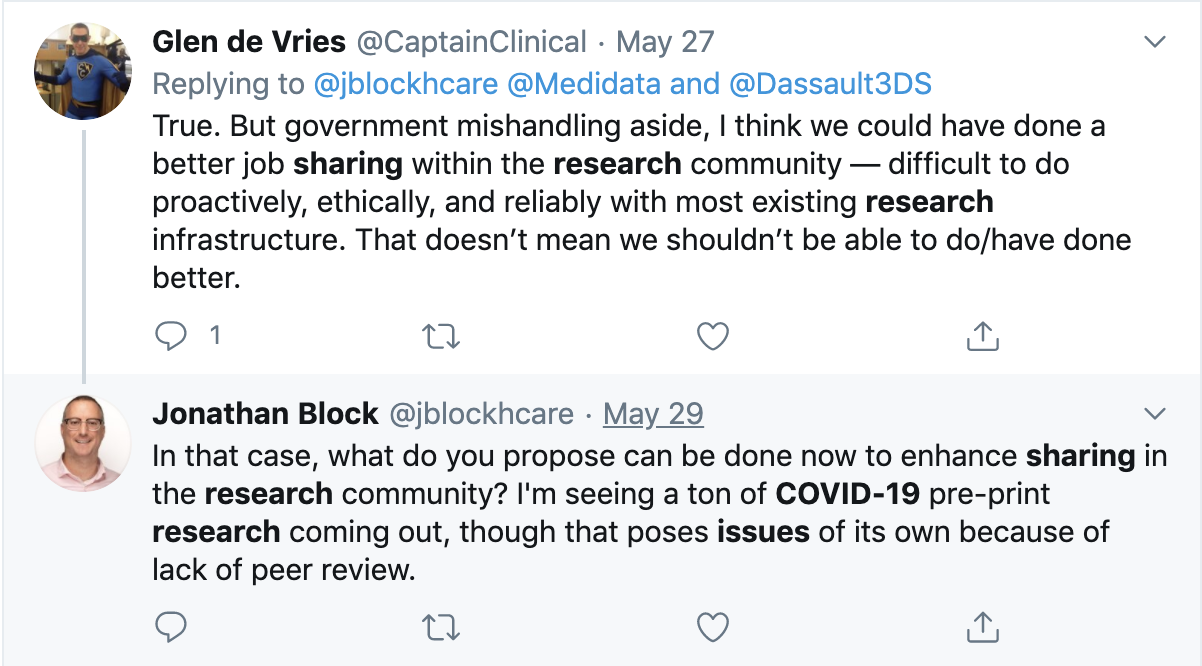
\includegraphics[width=0.5\textwidth]{Pictures/Appendix_Tweets/block and vries tweet.png}
  \caption{Jonathan Block replies to tweet by Glen de Vries about sharing research within the research community}
  \Description{Jonathan Block replies to tweet by Glen de Vries about sharing research within the research community}
  \label{block_vries_tweet}
\end{figure}

\begin{figure}
  
\includegraphics[width=0.5\textwidth]{Pictures/Appendix_Tweets/c michael gibson tweet.png}
  \caption{C. Michael Gibson tweets about surgisphere (a health analytics company) lying about collaborating with NHS Scotland}
  \Description{C. Michael Gibson tweets about surgisphere (a health analytics company) lying about collaborating with NHS Scotland}
  \label{c_michael_gibson_tweet}
\end{figure}

\begin{figure}
  
\includegraphics[width=0.5\textwidth]{Pictures/Appendix_Tweets/caitlin rivers tweet.png}
  \caption{Caitlin Rivers tweets the original WHO report on COVID-19 modes of transmission}
  \Description{Caitlin Rivers tweets the original WHO report on COVID-19 modes of transmission}
  \label{caitlin_rivers_tweet}
\end{figure}

\begin{figure}
  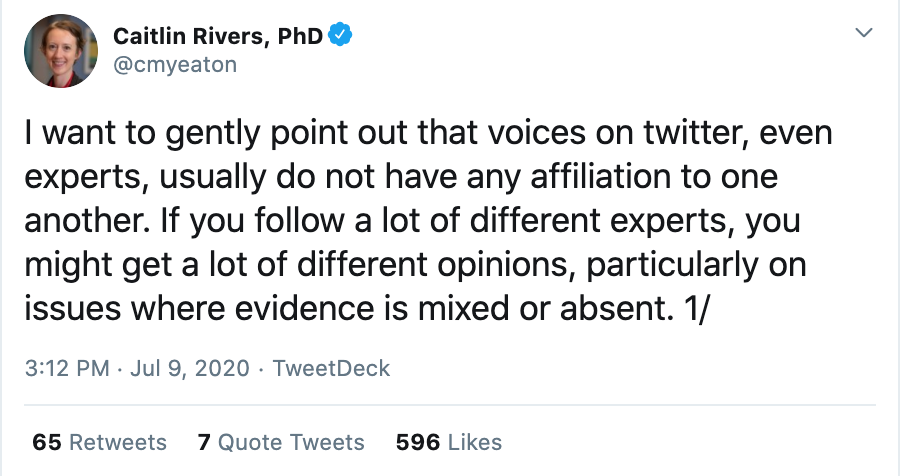
\includegraphics[width=0.5\textwidth]{Pictures/Appendix_Tweets/caitlin rivers tweet2.png}
  \caption{Dr.Caitlin Rivers tweets about the confusion led by many different expert opinions being shared on Twitter}
  \Description{Dr.Caitlin Rivers tweets about the confusion led by many different expert opinions being shared on Twitter}
  \label{caitlin_rivers_tweet2}
\end{figure}

\begin{figure}
  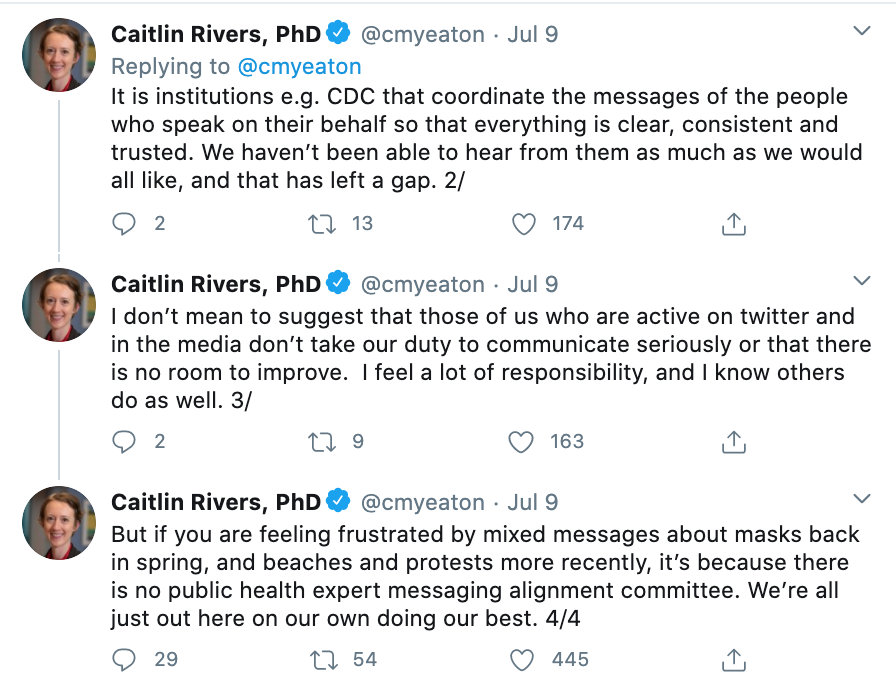
\includegraphics[width=0.5\textwidth]{Pictures/Appendix_Tweets/caitlin rivers tweet2 contd.png}
  \caption{Dr.Caitlin Rivers tweets about the confusion led by many different expert opinions being shared on Twitter}
  \Description{Dr.Caitlin Rivers tweets about the confusion led by many different expert opinions being shared on Twitter}
  \label{caitlin_rivers_tweet2_contd}
\end{figure}

\begin{figure}
  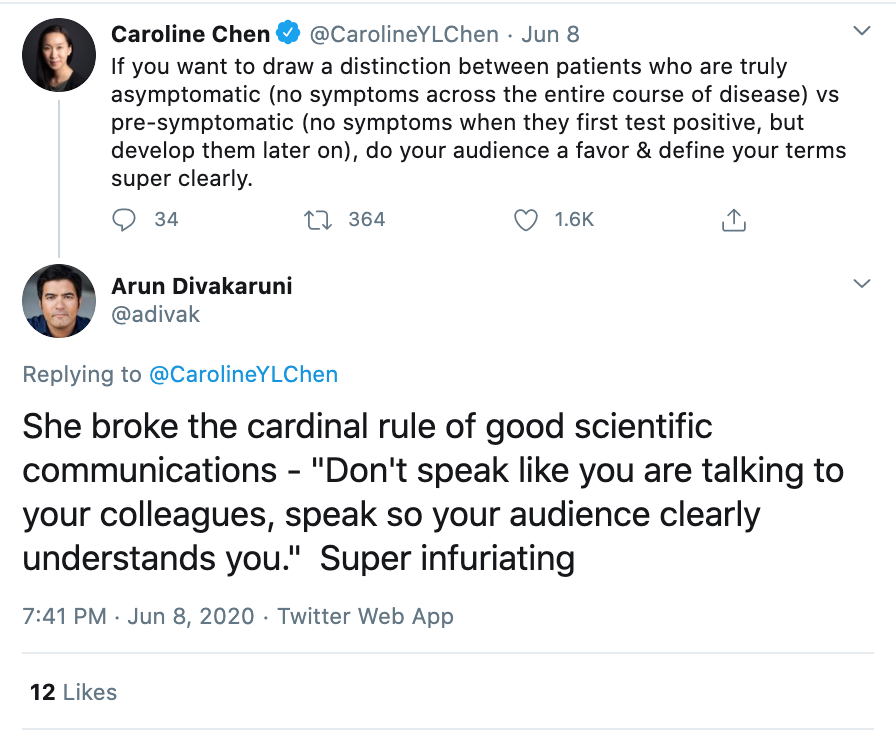
\includegraphics[width=0.5\textwidth]{Pictures/Appendix_Tweets/caroline chen and arun divakaruni tweet.png}
  \caption{Caroline Chen tweets about being clear and defining terminology when speaking to an audience as scientists and Arun Divakaruni replies in agreement}
  \Description{Caroline Chen tweets about being clear and defining terminology when speaking to an audience as scientists and Arun Divakaruni replies in agreement}
  \label{caroline_chen_tweet}
\end{figure}

\begin{figure}
  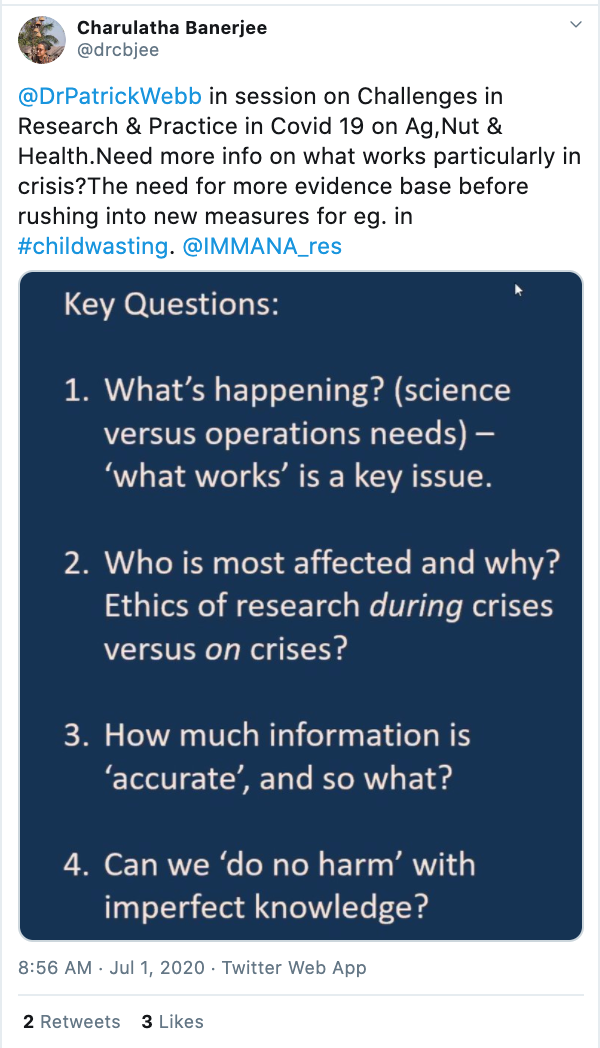
\includegraphics[width=0.5\textwidth]{Pictures/Appendix_Tweets/charulatha banerjee tweet.png}
  \caption{Charulatha Banerjee tweets about the need for more evidence base for publishing on COVID-19}
  \Description{Charulatha Banerjee tweets about the need for more evidence base for publishing on COVID-19}
  \label{charulatha_banerjee_tweet}
\end{figure}

\begin{figure}
  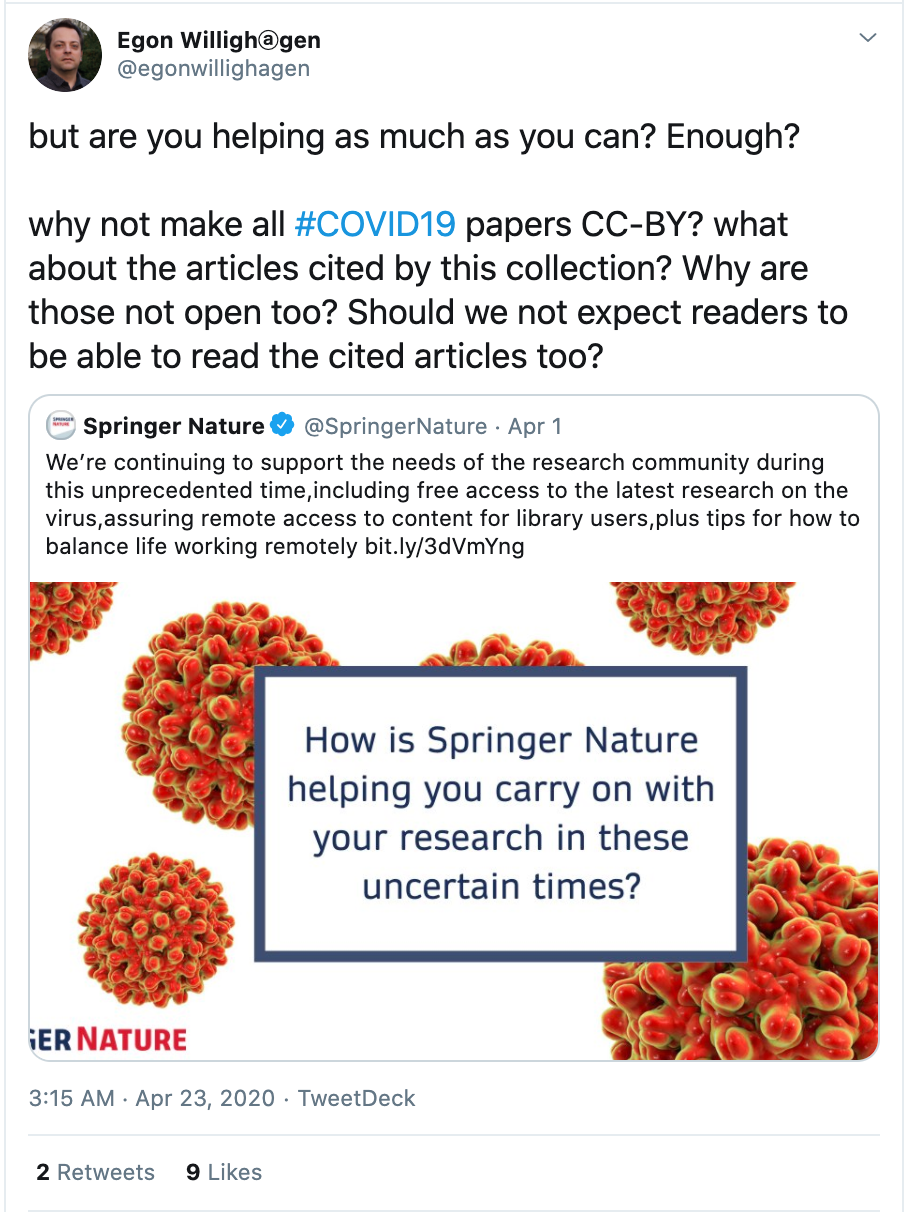
\includegraphics[width=0.5\textwidth]{Pictures/Appendix_Tweets/egon willighagen tweet.png}
  \caption{Egon Willighagen tweets about the inaccessibility to papers and their cited papers}
  \Description{Egon Willighagen tweets about the inaccessibility to papers and their cited papers}
  \label{egon_willighagen_tweet}
\end{figure}

\begin{figure}
  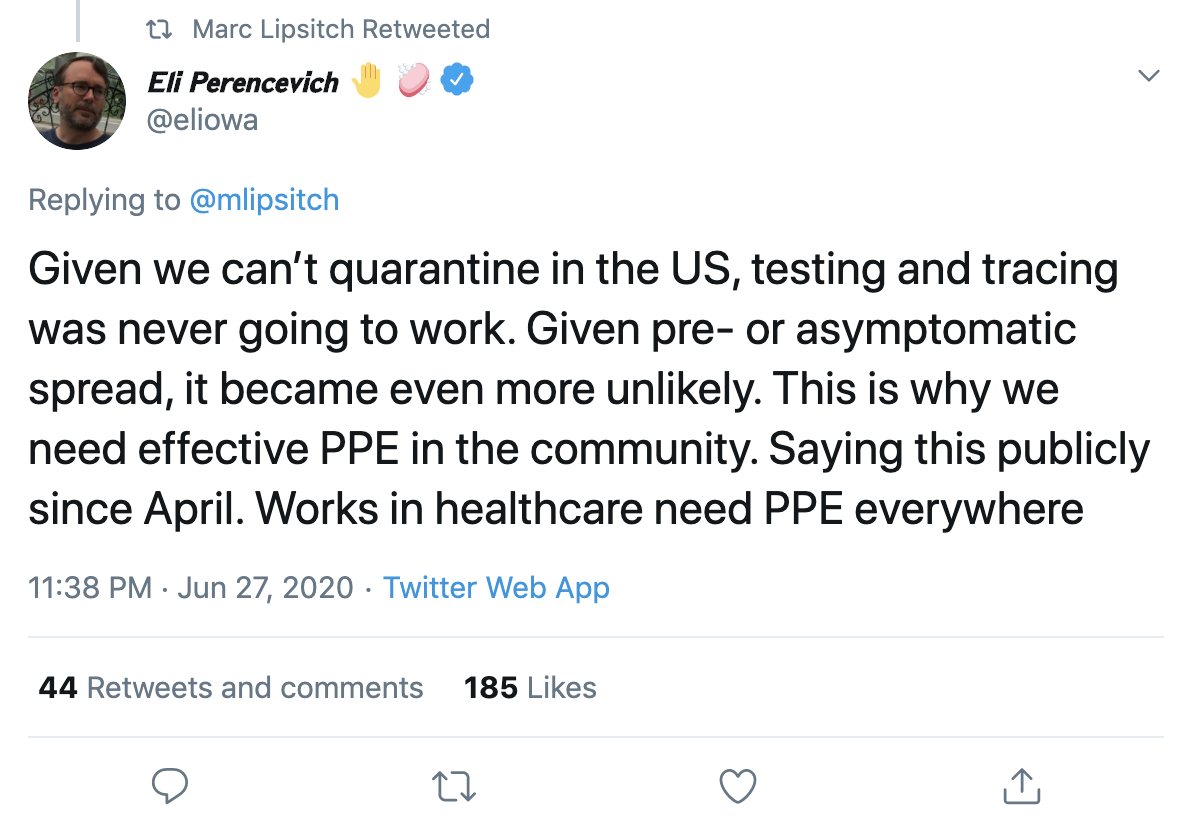
\includegraphics[width=0.5\textwidth]{Pictures/Appendix_Tweets/eli perencevich tweet.png}
  \caption{Eli Perencevich tweets about how he's been advocating for PPE since April}
  \Description{Eli Perencevich tweets about how he's been advocating for PPE since April}
  \label{eli_perencevich_tweet}
\end{figure}

\begin{figure}
  
\includegraphics[width=0.5\textwidth]{Pictures/Appendix_Tweets/ellie murray tweet.png}
  \caption{Ellie Murray tweets about precautions when sharing research findings}
  \Description{Ellie Murray tweets about precautions when sharing research findings}
  \label{ellie_murray_tweet}
\end{figure}

\begin{figure}
  
\includegraphics[width=0.5\textwidth]{Pictures/Appendix_Tweets/ellie murray tweet contd.png}
  \caption{Ellie Murray tweets about precautions when sharing research findings}
  \Description{Ellie Murray tweets about precautions when sharing research findings}
  \label{ellie_murray_tweet_contd}
\end{figure}

\begin{figure}
  
\includegraphics[width=0.5\textwidth]{Pictures/Appendix_Tweets/emma hodcroft tweet.png}
  \caption{Dr. Emma Hodcroft tweets that when a scientist points out that a paper doesn't have enough evidence, they are not saying it is wrong}
  \Description{Dr. Emma Hodcroft tweets that when a scientist points out that a paper doesn't have enough evidence, they are not saying it is wrong}
  \label{emma_hodcroft_tweet}
\end{figure}

\begin{figure}
  
\includegraphics[width=0.5\textwidth]{Pictures/Appendix_Tweets/gail carson tweet.png}
  \caption{Gail Carson tweets a call to action on responsible communication of scientific research}
  \Description{Gail Carson tweets a call to action on responsible communication of scientific research}
  \label{gail_carson_tweet}
\end{figure}

\begin{figure}
  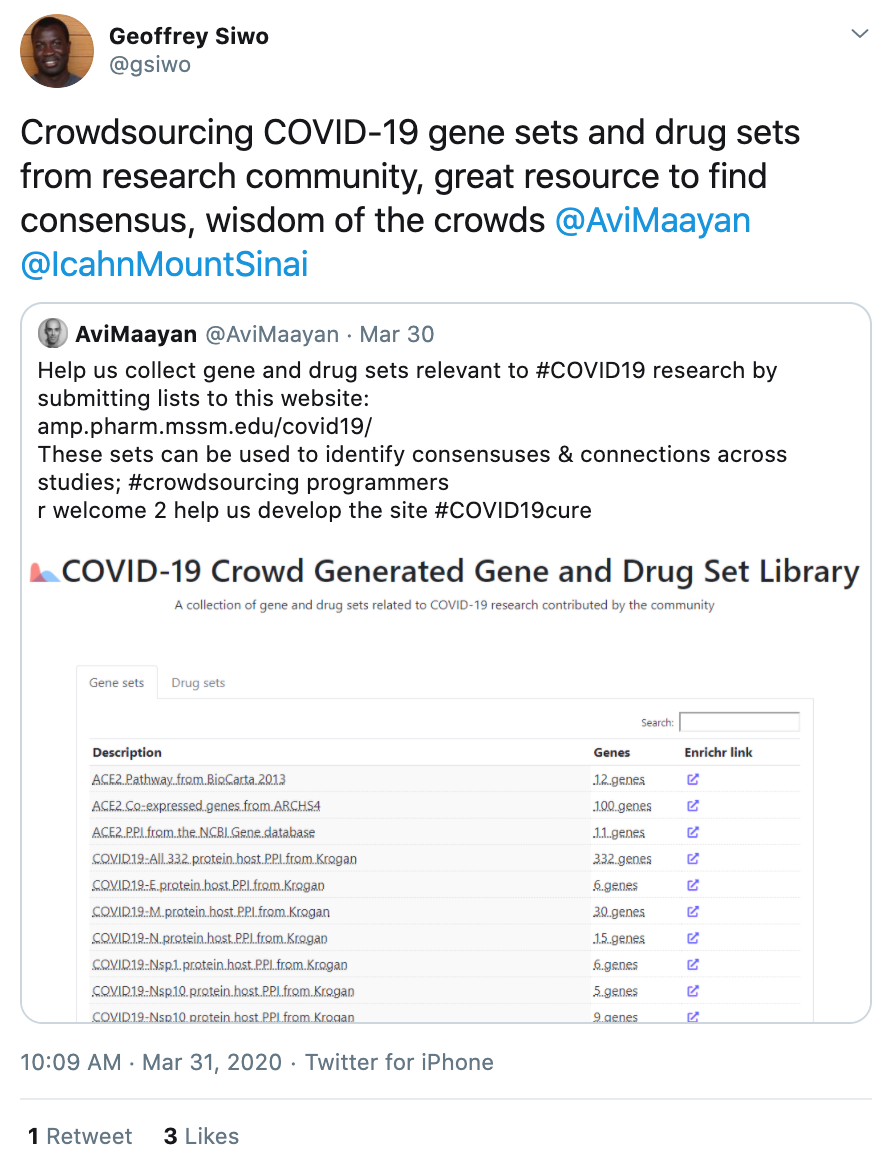
\includegraphics[width=0.5\textwidth]{Pictures/Appendix_Tweets/geoffrey siwo tweet.png}
  \caption{Geoffrey Siwo tweets about crowdsourced COVID-19 gene library that helps reach consensus}
  \Description{Geoffrey Siwo tweets about crowdsourced COVID-19 gene library that helps reach consensus}
  \label{geoffrey_siwo_tweet}
\end{figure}

\begin{figure}
  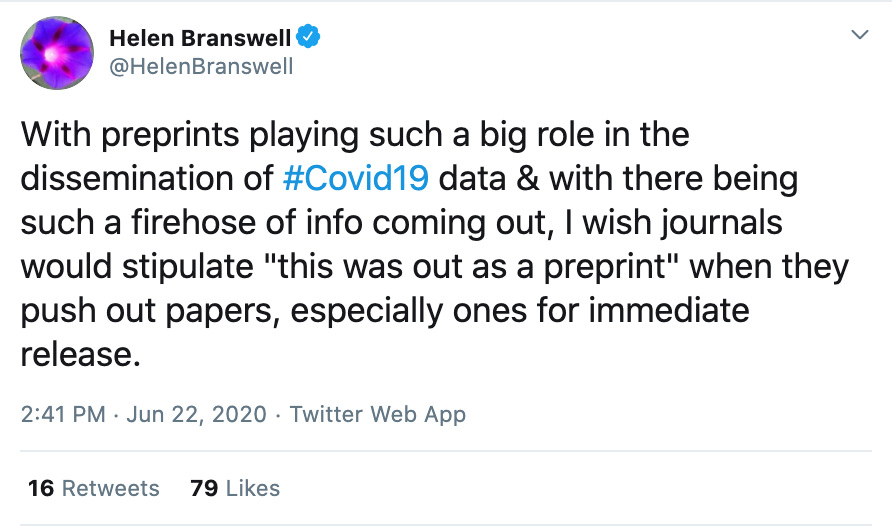
\includegraphics[width=0.5\textwidth]{Pictures/Appendix_Tweets/helen branswell tweet.png}
  \caption{Helen Branswell tweets about how journals should be clear about using COVID-19 preprints}
  \Description{Helen Branswell tweets about how journals should be clear about using COVID-19 preprints}
  \label{helen_branswell_tweet}
\end{figure}

\begin{figure}
  
\includegraphics[width=0.5\textwidth]{Pictures/Appendix_Tweets/james todaro tweet.png}
  \caption{James Todaros tweets about not finding a consensus on the IFR and current WHO estimates}
  \Description{James Todaros tweets about not finding a consensus on the IFR and current WHO estimates}
  \label{james_todaro_tweet}
\end{figure}

\begin{figure}
  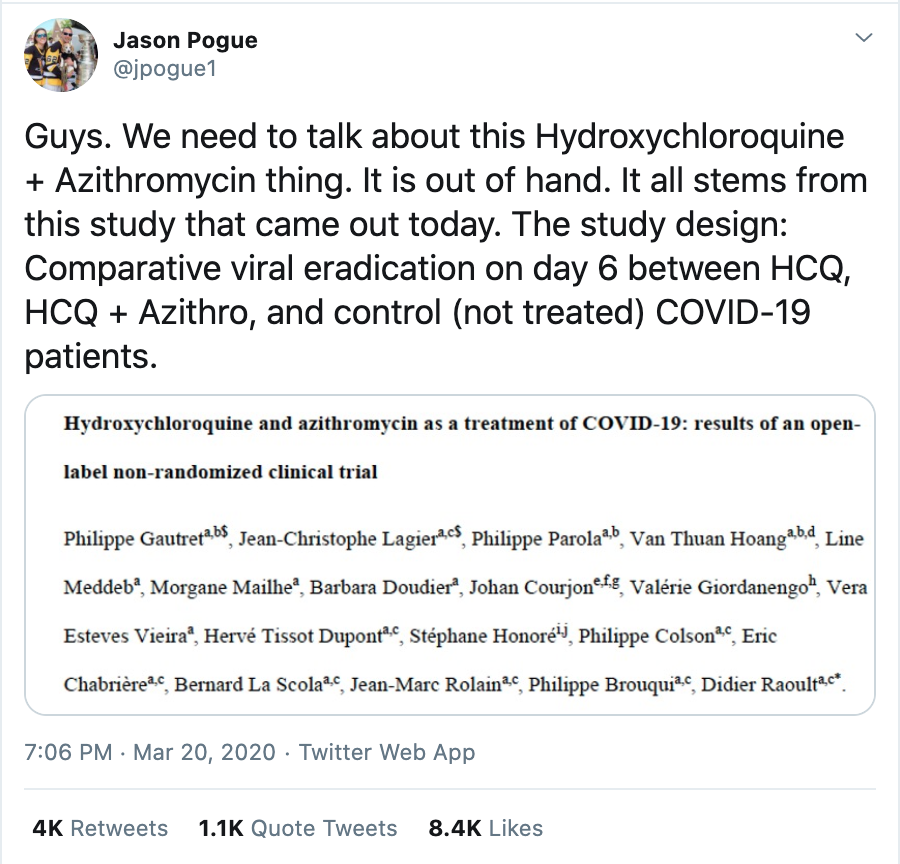
\includegraphics[width=0.5\textwidth]{Pictures/Appendix_Tweets/jason pogue tweet.png}
  \caption{James Pogue tweets about opening up a conversation on Hydroxychloroquine and Azithromycin}
  \Description{James Pogue tweets about opening up a conversation on Hydroxychloroquine and Azithromycin}
  \label{jason_pogue_tweet}
\end{figure}

\begin{figure}
  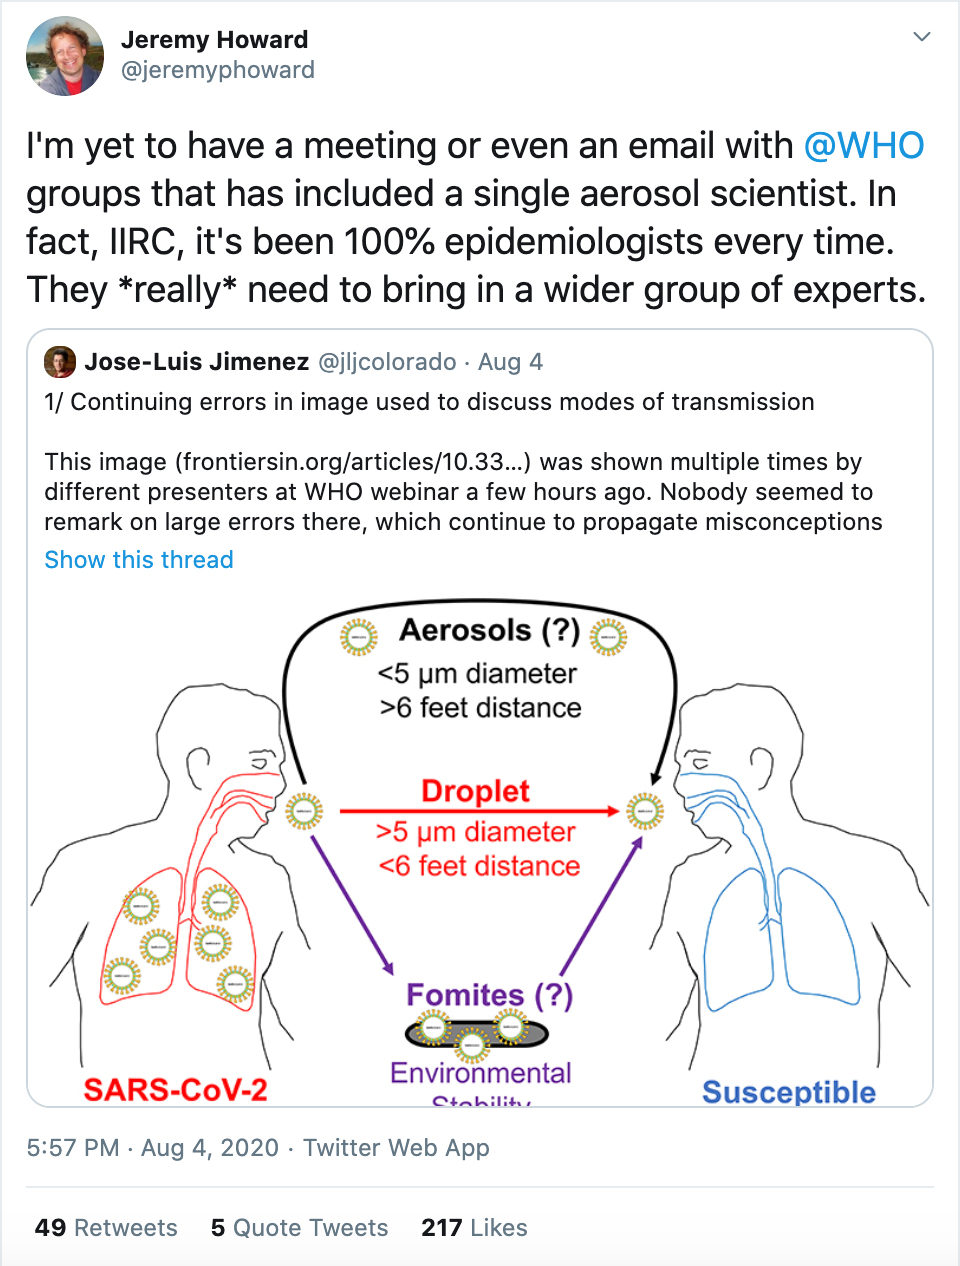
\includegraphics[width=0.5\textwidth]{Pictures/Appendix_Tweets/jeremy howard tweet.png}
  \caption{Jeremy Howard tweets about the lack of variety in experts at meetings}
  \Description{Jeremy Howard tweets about the lack of variety in experts at meetings}
  \label{jeremy_howard_tweet}
\end{figure}

\begin{figure}
  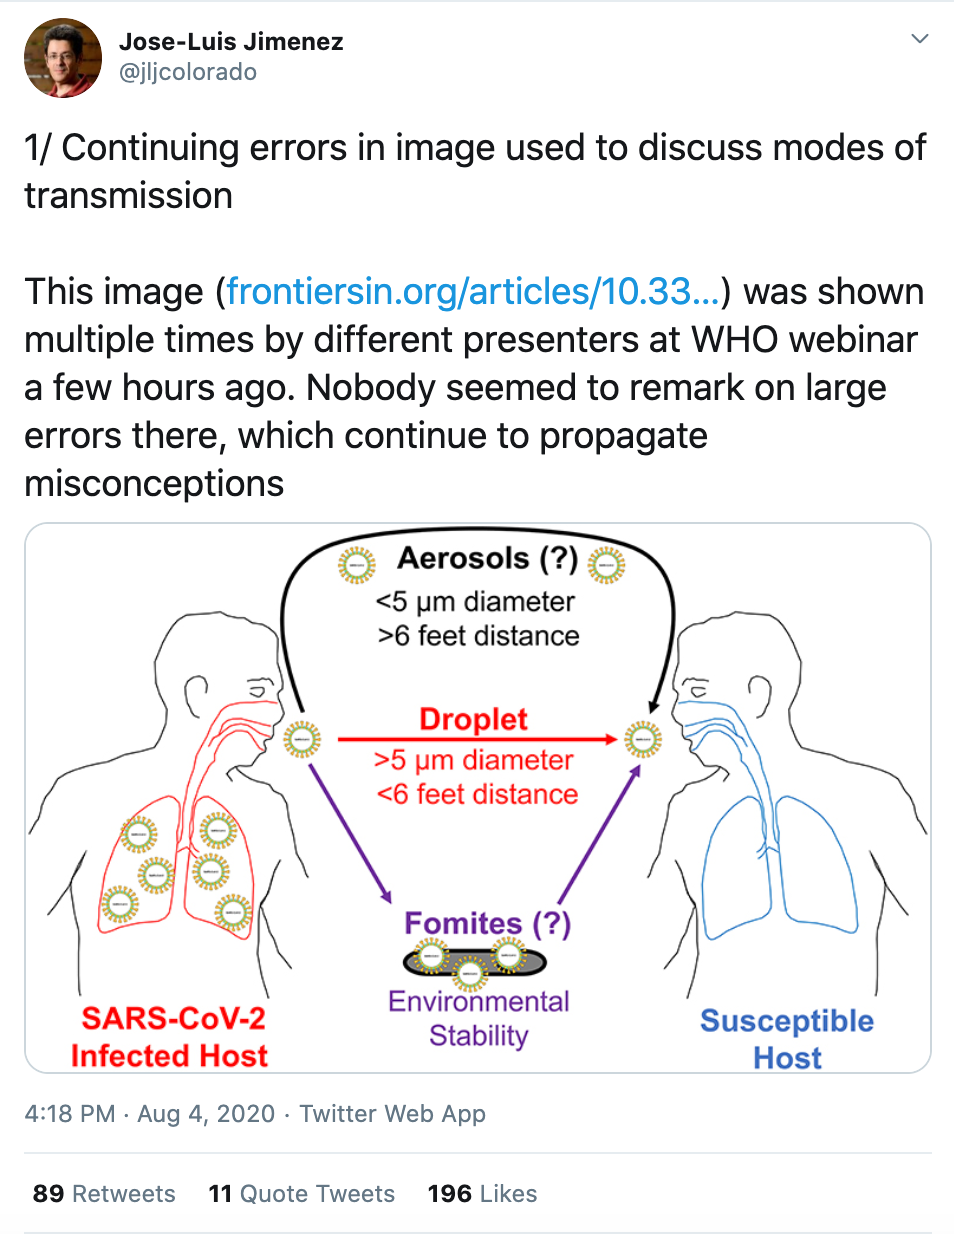
\includegraphics[width=0.5\textwidth]{Pictures/Appendix_Tweets/jose-luis jimenez tweet.png}
  \caption{Jose-Luis Jimenez tweets about errors in presentation slides talking about modes of transmission}
  \Description{Jose-Luis Jimenez tweets about errors in presentation slides talking about modes of transmission}
  \label{jose_luis_jimenez_tweet}
\end{figure}

\begin{figure}
  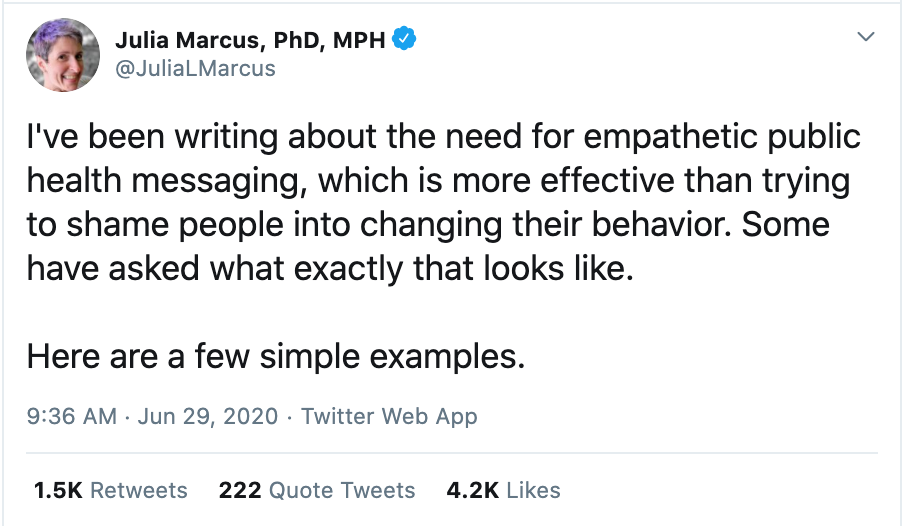
\includegraphics[width=0.5\textwidth]{Pictures/Appendix_Tweets/julie marcus tweet.png}
  \caption{Julie Marcus tweets about how public messaging should be more empathetic}
  \Description{Julie Marcus tweets about how public messaging should be more empathetic}
  \label{julie_marcus_tweet}
\end{figure}

\begin{figure}
  
\includegraphics[width=0.5\textwidth]{Pictures/Appendix_Tweets/kareem carr tweet.png}
  \caption{Kareem Carr tweets about unbalanced literature reviews}
  \Description{Kareem Carr tweets about unbalanced literature reviews}
  \label{kareem_carr_tweet}
\end{figure}

\begin{figure}
  
\includegraphics[width=0.5\textwidth]{Pictures/Appendix_Tweets/kareem carr tweet2.png}
  \caption{Kareem Carr tweets about science communication mistakes made by scientists}
  \Description{Kareem Carr tweets about science communication mistakes made by scientists}
  \label{kareem_carr_tweet2}
\end{figure}

\begin{figure}
  
\includegraphics[width=0.5\textwidth]{Pictures/Appendix_Tweets/kareem carr tweet2 contd.png}
  \caption{Kareem Carr tweets about science communication mistakes made by scientists}
  \Description{Kareem Carr tweets about science communication mistakes made by scientists}
  \label{kareem_carr_tweet2_contd}
\end{figure}

\begin{figure}
  
\includegraphics[width=0.5\textwidth]{Pictures/Appendix_Tweets/krutika kuppalli tweet.png}
  \caption{Krutika Kuppalli tweets about releasing data on media}
  \Description{Krutika Kuppalli tweets about releasing data on media}
  \label{krutika_kuppalli_tweet}
\end{figure}

\begin{figure}
  
\includegraphics[width=0.5\textwidth]{Pictures/Appendix_Tweets/maria tapia tweet.png}
  \caption{Maria Tapia tweets about the importance of vocabulary in science}
  \Description{Maria Tapia tweets about the importance of vocabulary in science}
  \label{maria_tapia_tweet}
\end{figure}

\begin{figure}
  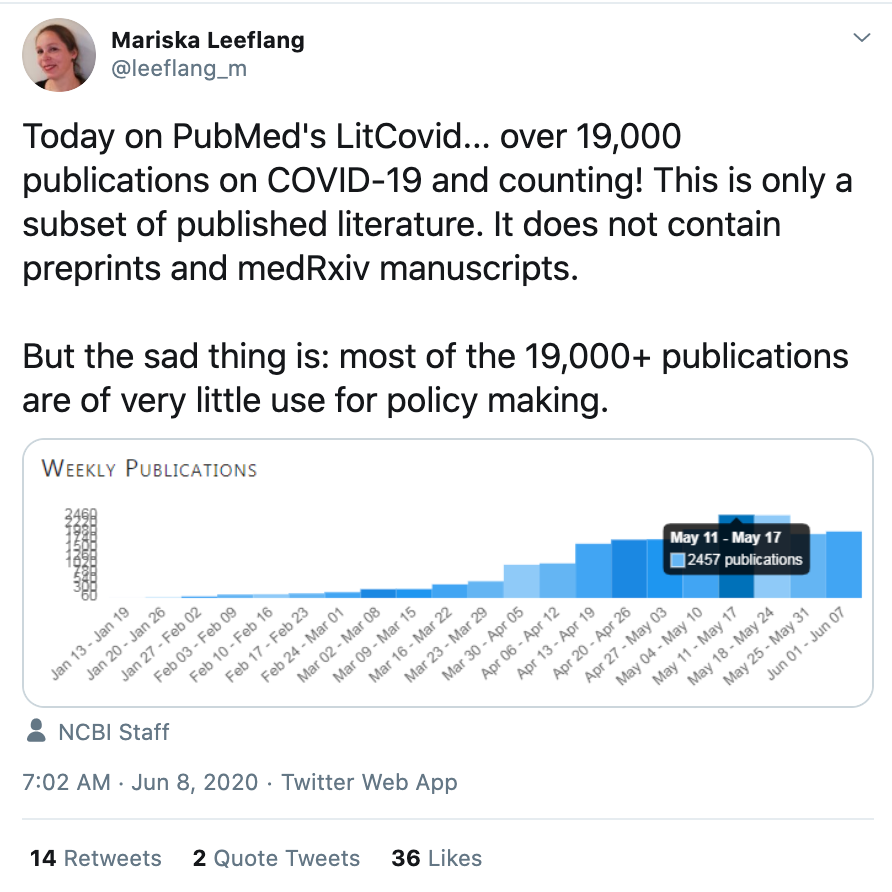
\includegraphics[width=0.5\textwidth]{Pictures/Appendix_Tweets/mariska leefland tweet.png}
  \caption{Mariska Leefland tweets about how many COVID papers are being published but they are making little policy difference}
  \Description{Mariska Leefland tweets about how many COVID papers are being published but they are making little policy difference}
  \label{mariska_leefland_tweet}
\end{figure}

\begin{figure}
  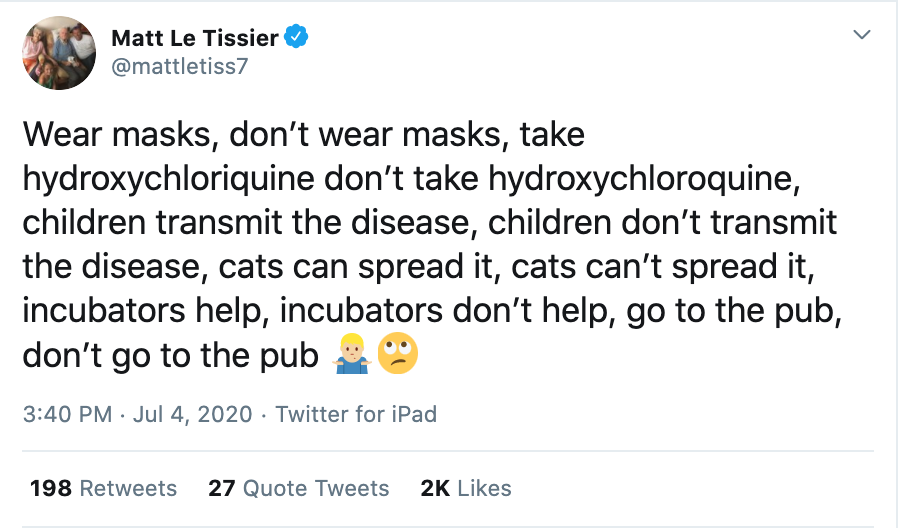
\includegraphics[width=0.5\textwidth]{Pictures/Appendix_Tweets/matt le tissier tweet.png}
  \caption{Matt Le Tissier tweets about the contradictions in inscientist point of views on COVID-19}
  \Description{Matt Le Tissier tweets about the contradictions in inscientist point of views on COVID-19}
  \label{matt_le_tissier_tweet}
\end{figure}

\begin{figure}
  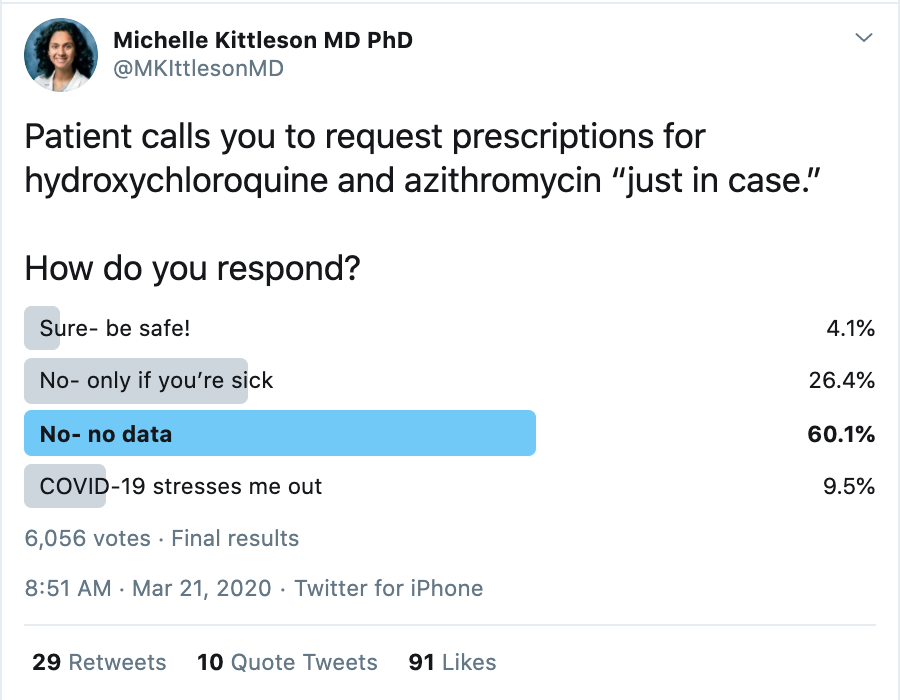
\includegraphics[width=0.5\textwidth]{Pictures/Appendix_Tweets/michelle kittleson tweet.png}
  \caption{Michelle Kittleson tweets a poll of how people respond to request for hydroxychloroquine}
  \Description{Michelle Kittleson tweets a poll of how people respond to request for hydroxychloroquine}
  \label{michelle_kittleson_tweet}
\end{figure}

\begin{figure}
  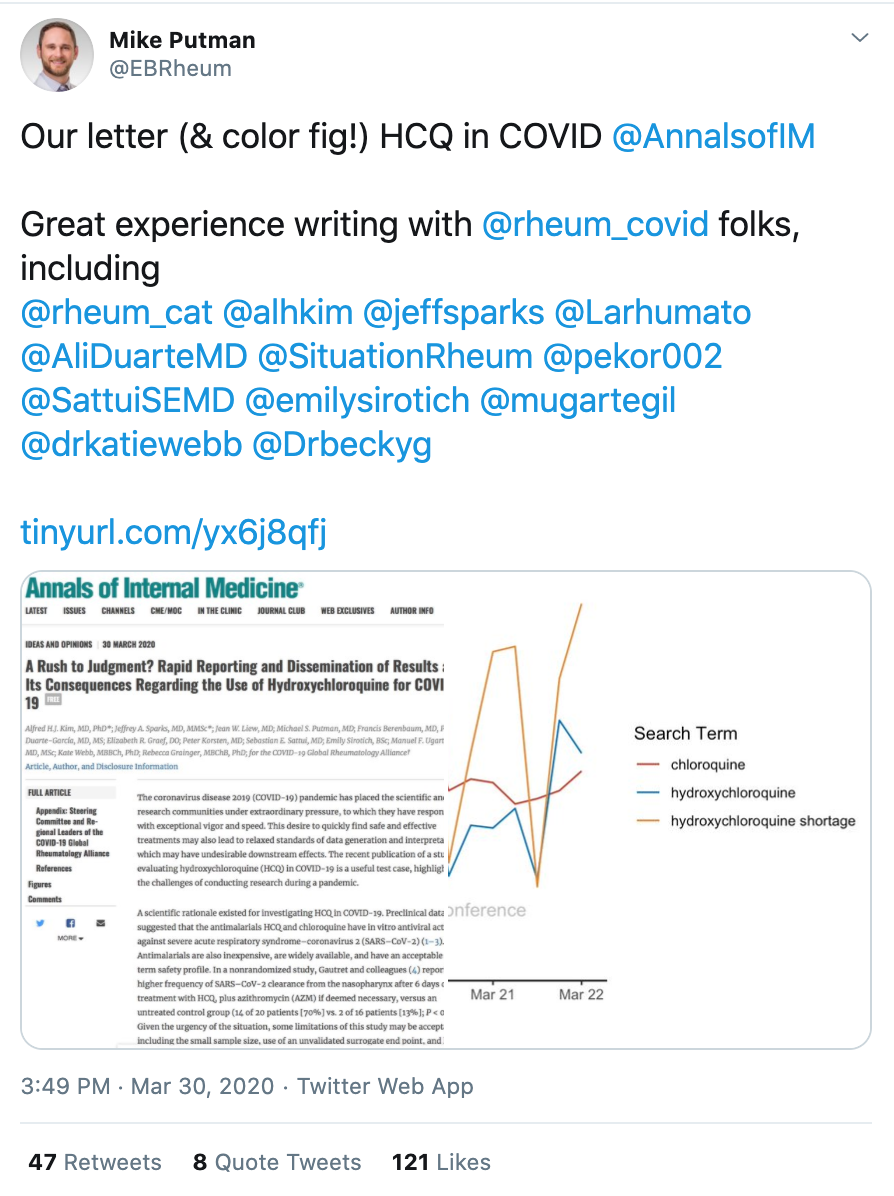
\includegraphics[width=0.5\textwidth]{Pictures/Appendix_Tweets/mike putman tweet.png}
  \caption{Mike Putman tweets a letter they wrote on Hydroxychloroquine in COVID-19}
  \Description{Mike Putman tweets a letter they wrote on Hydroxychloroquine in COVID-19}
  \label{mike_putman_tweet}
\end{figure}

\begin{figure}
  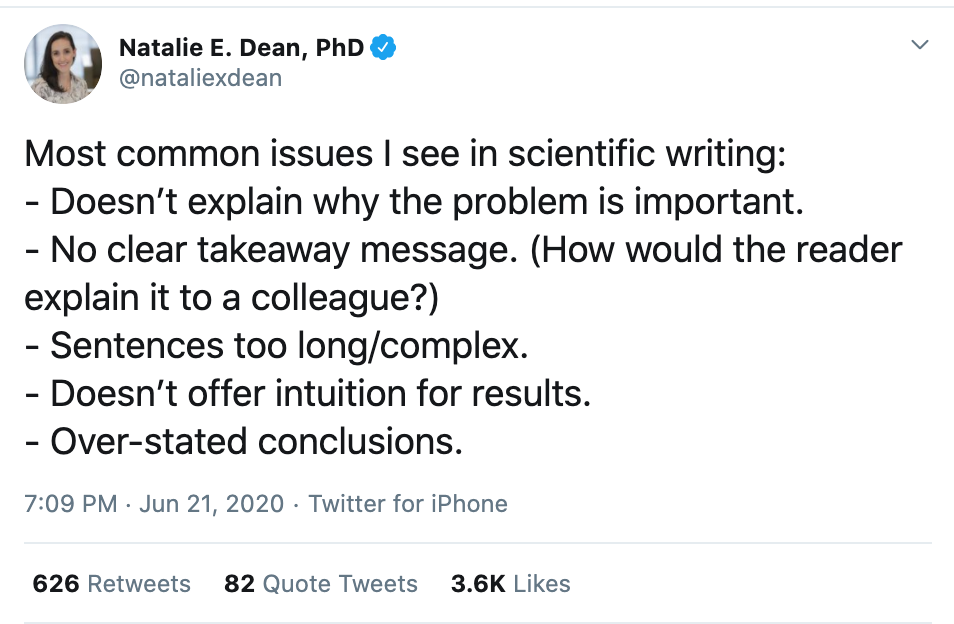
\includegraphics[width=0.5\textwidth]{Pictures/Appendix_Tweets/natalie dean tweet.png}
  \caption{Natalie Dean tweets about the issues seen in scientific writing}
  \Description{Natalie Dean tweets about the issues seen in scientific writing}
  \label{natalie_dean_tweet}
\end{figure}

\begin{figure}
  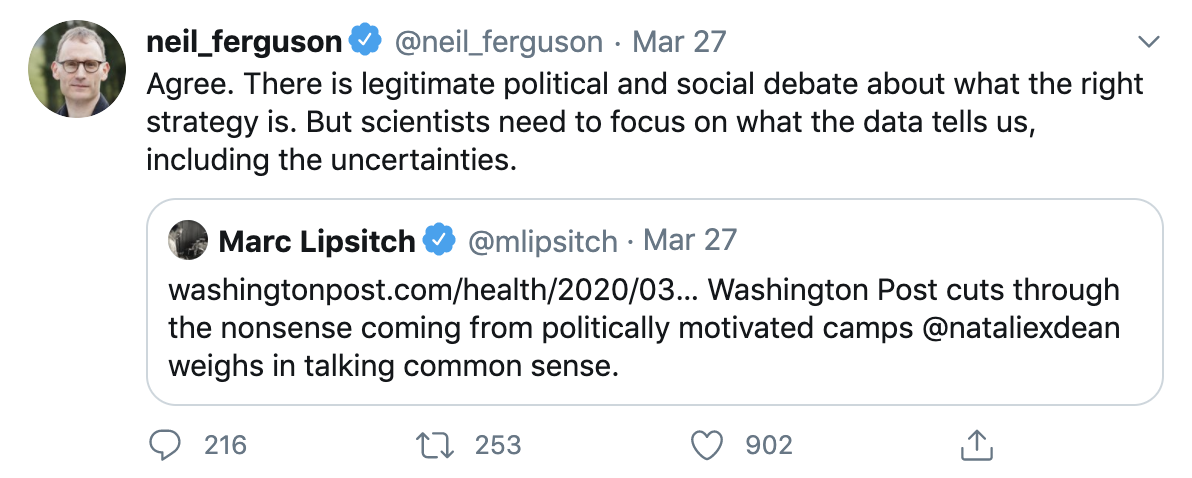
\includegraphics[width=0.5\textwidth]{Pictures/Appendix_Tweets/neil ferguson tweet.png}
  \caption{Neil Ferguson tweets about focusing on uncertainties as scientists}
  \Description{Neil Ferguson tweets about focusing on uncertainties as scientists}
  \label{neil_fergusen}
\end{figure}

\begin{figure}
  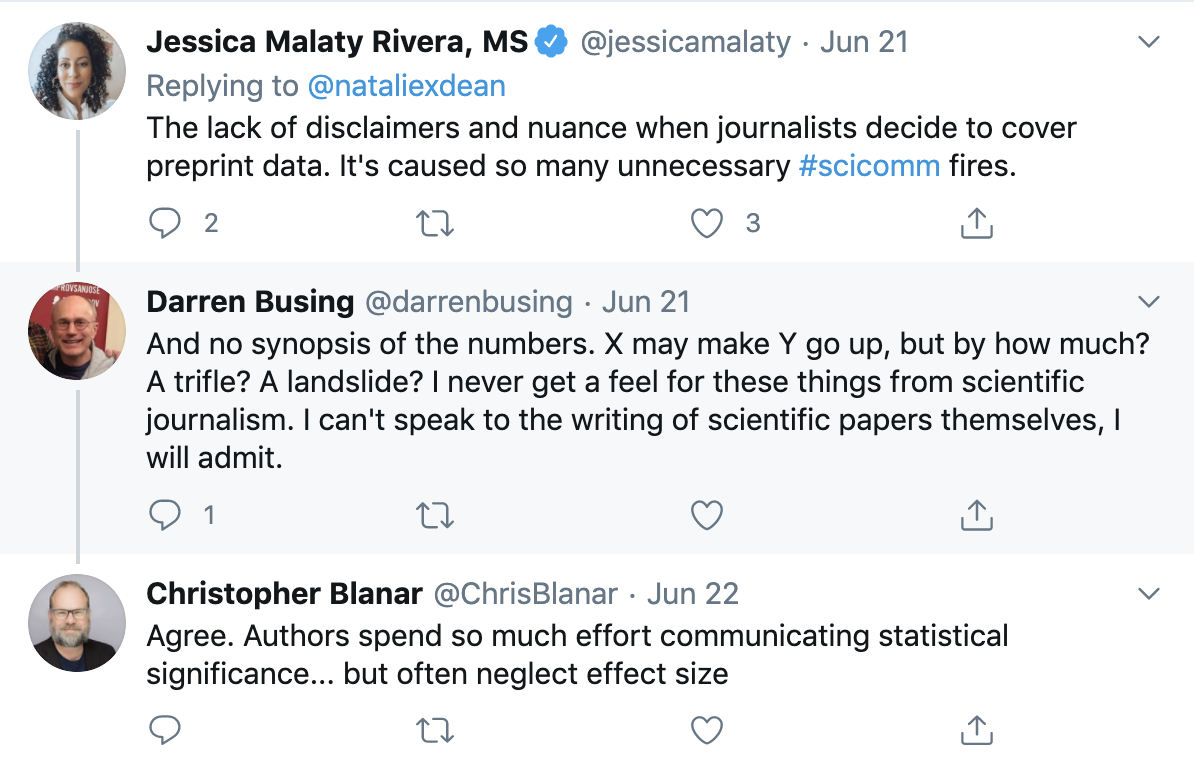
\includegraphics[width=0.5\textwidth]{Pictures/Appendix_Tweets/revera tweet.png}
  \caption{Jessica Malaty Rivera tweets about the coverage of preprints}
  \Description{Jessica Malaty Rivera tweets about the coverage of preprints}
  \label{revera_tweet}
\end{figure}

\begin{figure}
  \includegraphics[width=0.5\textwidth]{Pictures/Appendix_Tweets/roberto rocha tweet.png}
  \caption{Roberto Rocha has a twitter thread on the conversation between scientists on finding a consensus about COVID-19}
  \Description{Roberto Rocha has a twitter thread on the conversation between scientists on finding a consensus about COVID-19}
  \label{roberto_rocha_tweet}
\end{figure}

\begin{figure}
  \includegraphics[width=0.5\textwidth]{Pictures/Appendix_Tweets/saskia popescu tweet.png}
  \caption{Dr.Saskia Popescu tweets about evolving data}
  \Description{Dr.Saskia Popescu tweets about evolving data}
  \label{saskia_popescu_tweet}
\end{figure}

\begin{figure}
  \includegraphics[width=0.5\textwidth]{Pictures/Appendix_Tweets/saskia popescu tweet2.png}
  \caption{Dr.Saskia Popescu tweets about how the term ``airborne'' is communicated by scientists}
  \Description{Dr.Saskia Popescu tweets about how the term ``airborne'' is communicated by scientists}
  \label{saskia_popescu_tweet2}
\end{figure}

\begin{figure}
  \includegraphics[width=0.5\textwidth]{Pictures/Appendix_Tweets/saskia popescu tweet2 contd.png}
  \caption{Dr.Saskia Popescu tweets about how the term ``airborne'' is communicated by scientists}
  \Description{Dr.Saskia Popescu tweets about how the term ``airborne'' is communicated by scientists}
  \label{saskia_popescu_tweet2_contd}
\end{figure}

\begin{figure}
  \includegraphics[width=0.5\textwidth]{Pictures/Appendix_Tweets/soragni lab tweet.png}
  \caption{Soragni:Lab tweets their thoughts on experts from unrelated fields with no relevant expertise contributing to COVID-19 research}
  \Description{Soragni:Lab tweets their thoughts on experts from unrelated fields with no relevant expertise contributing to COVID-19 research}
  \label{soragni_lab_tweet}
\end{figure}

\begin{figure}
  \includegraphics[width=0.5\textwidth]{Pictures/Appendix_Tweets/steven nono tweet.png}
  \caption{Steven \~{N}o\~{n}o tweets about the lack of science communication among COVID-19 researchers}
  \Description{Steven \~{N}o\~{n}o tweets about the lack of science communication among COVID-19 researchers}
  \label{steven_nono_tweet}
\end{figure}

\begin{figure}
  \includegraphics[width=0.5\textwidth]{Pictures/Appendix_Tweets/trevor bedford tweet.png}
  \caption{Trevor Bedford tweets about a Twitter space whose function is no longer about hosting conversations but is now about outreach}
  \Description{Trevor Bedford tweets about a Twitter space whose function is no longer about hosting conversations but is now about outreach}
  \label{trevor_bedford_tweet}
\end{figure}


\end{document}
\endinput
%%
%% End of file `sample-authordraft.tex'.
